\chapter{Измерение импульсного отклика акустического MLS-сигнала в среде с потоком}

\section{Введение}
В данное время широко используемым методом измерения импульсных откликов и частотных характеристик различных акустических рассеивателей является техника измерения импульсного отклика с помощью псевдослучайной последовательности максимальной длины (Maximum Length Sequence) \cite{ValyaevMLS, ValyaevRoad, Denisov2017}. Суть техники заключается в зондировании испытуемой системы квазишумовой посылкой, автокорреляционная функция которой близка к дельта-функции, и последующей корреляционной обработке полученных данных.

Ценность дифракционного MLS-эксперимента состоит в возможности непосредственного наблюдения полей, дифрагированных на различных, в том числе и сложных, объектах. В данной работе ставится практически важная задача применить технику MLS-эксперимента в случае прохождения акустического сигнала через воздушную струю.

Эксперименты по изучению воздушных струй акустическими методами уже проводились и описаны в существующих работах. В \cite{Candel1976} изучается экранирование струей монохроматического сигнала в зависимости от взаимных ориентаций струи и источника сигнала. Аналитическая модель этого процесса предложена в \cite{Gerhold1983}. Вопрос о поведении фазы акустической волны при прохождении через турбулентный поток численно рассмотрен в \cite{Karweit1991}. Экспериментальное изучение случайных характеристик струи на основе поведения монохроматической акустической волны, проходящей через струю перпендикулярно направлению потока, проведено в \cite{HoChi}.
 
Имеются и работы по изучению влияния акустических волн на потоки воздуха с небольшими скоростями \cite{Golovanov2006, Vlasov1971}. В данной работе такое влияние не рассматривается.

Кроме того, имеется множество работ, посвященных отражению и прохождению акустических волн через тангенциальный разрыв на плоской границе двух движущихся жидкостей \cite{Friedland1969, Godin1988, Jones1973, Gottlieb1960}. 

В \cite{Ahuja1981} описаны эксперименты по корреляционному детектированию широкополосного сигнала, проходящего через воздушную струю. В первом из них точечный источник помещался на оси потока, рядом с ним располагался контрольный микрофон, а снаружи потока размещался измерительный микрофон. По корреляции между сигналами с микрофонов определялась задержка прохождения сигнала и, соответственно, угол рефракции на границе потока. Во втором эксперименте источник с контрольным микрофоном также находится на оси потока, а два измерительных располагаются вне потока и на оси потока ниже по течению. Рассматривая поток, как отличную от воздуха среду, авторы измеряют и моделируют углы преломления и отражения на границе поток-пространство. 

В данной работе с помощью монопольного источника и MLS-техники \cite{ValyaevMLS, ValyaevRoad, Denisov2017} производится экспериментальное измерение импульсного отклика при наличии потока на акустической трассе. Изучаются явления сноса сигнала потоком и фокусировки сигнала цилиндрической струей. Проводится математическое моделирование этого процесса путем решения уравнения для распространения звука в постоянном потоке \cite{Blokhitsev1981} методом конечных разностей.

\section{Описание эксперимента}
Эксперименты проводились в заглушенной камере с потоком АК-2 ЦАГИ. Схема эксперимента показана на (Рис. \ref{img:ris2_1}). На рисунке показана система координат $(x,y,z)$, используемая ниже для задания положений микрофонов и источника.

Поток воздуха со скоростями $20, 40, 60, 80$ м/с создавался соплом круглого сечения диаметром $40$ см. На некотором расстоянии от сопла были расположены $3$ микрофона и источник звука, так чтобы акустическая трасса проходила через струю (Рис. \ref{img:ris2_1}). Была проведена серия экспериментов, в которых акустическая трасса была как перпендикулярна (Рис. \ref{img:ris2_2}), так и неперпендикулярна оси потока (Рис. \ref{img:ris2_3}).

\begin{figure}[ht]
	\centering
	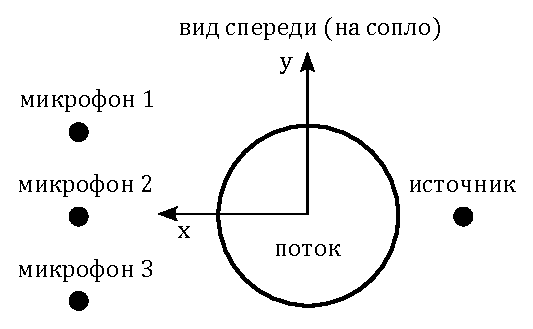
\includegraphics [scale=1] {ris2_1}
	\caption{Схема эксперимента с потоком.}
	\label{img:ris2_1}
\end{figure}

\begin{figure}[ht]
	\centering
	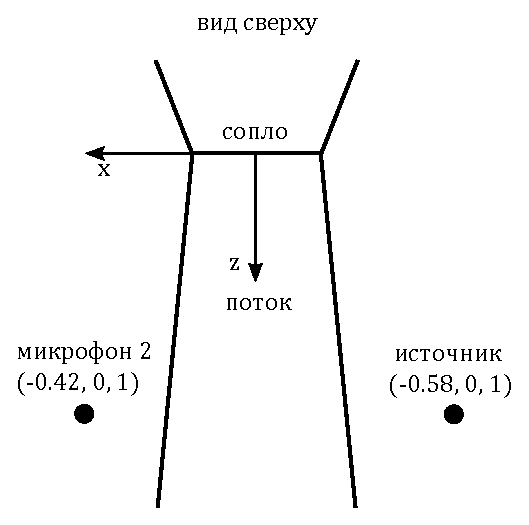
\includegraphics [scale=1] {ris2_2}
	\caption{Геометрия эксперимента. Акустическая трасса перпендикуляра оси потока.}
	\label{img:ris2_2}
\end{figure}

\begin{figure}[ht]
	\centering
	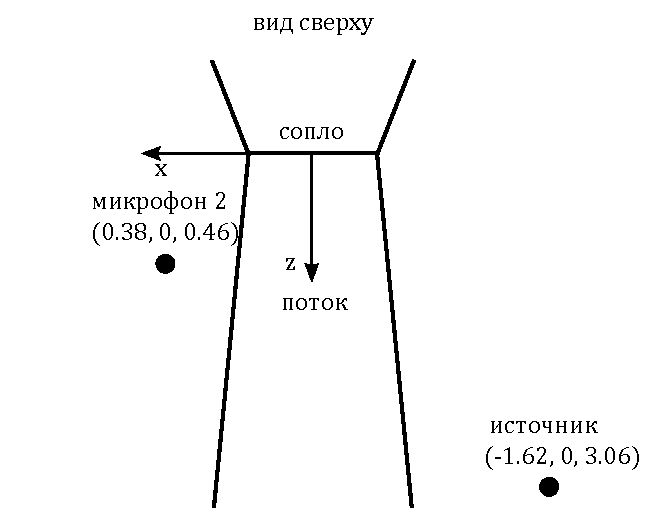
\includegraphics [scale=1] {ris2_3}
	\caption{Геометрия эксперимента. Акустическая трасса неперпендикулярна оси потока.}
	\label{img:ris2_3}
\end{figure}

Экспериментальное оборудование и алгоритм корреляционной обработки данных были аналогичны таковым, описанным в \cite{ValyaevMLS, ValyaevRoad, Denisov2017}. В качестве источника использовался всенаправленный излучатель Omnisource тип 4295 фирмы Bruel \& Kjaer с датчиком объемной скорости, в качестве микрофонов применялись ¼-дюймовые микрофоны типа 4935 фирмы Bruel \& Kjaer.

\section{Теоретическое описание}
Полноценное описание волновых процессов в среде с потоком было дано в \cite{Blokhitsev1981}. В данной монографии указывается, что скорость потока может быть представлена в виде средней скорости и флуктуации. Средняя скорость обуславливает снос и фокусировку звуковой волны, а переменная часть скорости ведет к рассеянию звука на флюктуациях. Для описания эффектов, связанных с переменной составляющей потока, необходимы данные о масштабах флуктуаций его скорости. Измерения этих масштабов в настоящей работе не производились. Ниже будет дано теоретическое описание эффектов, обусловленных постоянной составляющей потока.

\subsection{Расчет сноса звукового поля}
Для оценки сноса акустического сигнала будем рассматривать упрощенную двумерную (в координатах $x, z$ ) модель (Рис. \ref{img:ris2_4}). Будем считать, что скорость потока постоянна внутри струи и равна нулю за её пределами. Тогда, акустический потенциал $\Phi$  удовлетворяет уравнению \cite{Blokhitsev1981}:

\begin{equation}
\label{eq:2_1}
\left(\frac{\partial^2}{\partial x^2} + \frac{\partial^2}{\partial z^2}\right) \Phi = \left(M \frac{\partial}{\partial z} + \frac{1}{c} \frac{\partial}{\partial t}\right)^2 \Phi,
\end{equation}
где $M = V/c$ – число Маха, а $V$ – скорость потока. Здесь подразумевается, что $M$ постоянно внутри потока и равно нулю снаружи. Для корректной постановки задачи накладываются условия непрерывности давления и нормальной компоненты скорости на границе.
Используя принцип локальности \cite{Keller1962}, выпишем представление акустического потенциала звукового поля на приемнике в виде фазового интеграла, полученного в \cite{Mironov1975}: 

\begin{equation}
\label{eq:2_2}
\Phi = \int \int A(\omega) \exp(i f (\omega, k_z)) d\omega dk_z,
\end{equation}

\begin{equation}
\label{eq:2_3}
f(\omega, k_z) = -\omega t + k_z(z_2 - z_1) + (x_2 - x_1 - H) \sqrt{\frac{\omega^2}{c^2} - k_z^2} + H\sqrt{\left(\frac{\omega}{c} - Mk_z\right)^2 - k_z^2}
\end{equation}

Этот интеграл получен в результате применения преобразования Фурье к уравнению ~\eqref{eq:2_1} по времени и по координате $z$, направленной вдоль потока. В функции $f$ ~\eqref{eq:2_3} третий член описывает распространение вдоль оси $x$ в пространстве без потока, а четвертый член описывает распространение в пространстве с потоком. 

\begin{figure}[ht]
	\centering
	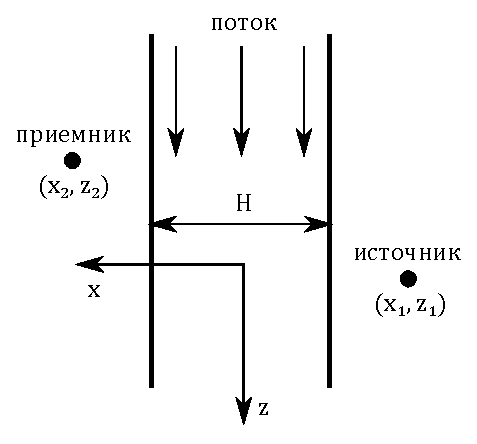
\includegraphics [scale=1] {ris2_4}
	\caption{Двухмерная модель.}
	\label{img:ris2_4}
\end{figure}

В случаях, когда длины волн меньше характерных масштабов неоднородностей, для анализа фазовых интегралов обычно применяют метод стационарной фазы или метод перевала \cite{SveshnikovTFKP}. В рассматриваемом случае интеграла ~\eqref{eq:2_2} необходимо применять метод стационарной фазы для двух комплексных переменных, для чего в комплексной плоскости переменных $(\omega, k_z)$ необходимо отыскать стационарные точки, в которых для подынтегральной функции выполняются условия.

\begin{equation}
\label{eq:2_4}
\frac{\partial f}{\partial \omega} = 0, \quad \frac{\partial f}{\partial k_z} = 0.
\end{equation}

В окрестностях стационарных точек осцилляции подынтегральной функции замедляются, и поэтому эти точки дают существенный вклад в интеграл, а в окрестности остальных точек подынтегральная функция быстро осциллирует, и поэтому такие окрестности не дают существенного вклада в интеграл.

Введем переменную $\gamma = k_z/(\omega/c)$  и перепишем ~\eqref{eq:2_3} в виде:

\begin{equation}
\label{eq:2_5}
f(\omega, \gamma) = \omega \left[-t + \frac{\gamma(z_2 - z_1)}{c} + \frac{x_2 - x_1 - H}{c} \sqrt{1 - \gamma^2} + \frac{H}{c} \sqrt{(1 - M\gamma)^2 - \gamma^2}\right]
\end{equation}

Условия ~\eqref{eq:2_4} перепишутся как 

\begin{equation}
\label{eq:2_6}
\frac{\partial f}{\partial \omega} = 0, \quad \frac{\partial f}{\partial \gamma} = 0,
\end{equation}
т.е.
\begin{equation}
\label{eq:2_7}
t = \frac{\gamma_* (z_2 - z_1)}{c} + \frac{x_2 - x_1 - H}{c} \sqrt{1 - \gamma_*^2} + \frac{H}{z} \sqrt{(1 - M\gamma_*)^2 - \gamma_*^2}
\end{equation}
где $\gamma_*$ - корень уравнения 
\begin{equation}
\label{eq:2_8}
(z_2 - z_1) - (x_2 - x_1 - H) \frac{\gamma}{\sqrt{1 - \gamma^2}} - H \frac{\gamma + M(1 - M \gamma)}{\sqrt{(1 - M\gamma)^2 - \gamma^2}} = 0.
\end{equation}

Решения уравнений ~\eqref{eq:2_7} и ~\eqref{eq:2_8} дают оценку времени прихода сигнала.

В общем случае время прихода сигнала $t$ для случая с потоком будет отличаться от времени распространения сигнала при отсутствии потока. Причина этого физически очевидна – часть времени сигнал распространяется против потока, что уменьшает фазовую скорость сигнала. В случае распространения звука по потоку время прохождения сигнала уменьшится. В данной работе случай ускорения звука не рассматривается, и соответствующий эксперимент проведен не был. 

\subsection{Расчет фокусировки звукового поля}

Если проекция единичного вектора вдоль звукового луча на скорость потока отрицательна, то фазовая скорость сигнала, распространяющегося вдоль такого луча, уменьшается, и, тем самым, поток может рассматриваться как акустически менее плотная среда.  В этом случае цилиндрический поток выступает как собирающая линза. Схема фокусировки показана на (Рис. \ref{img:ris2_6}).

\begin{figure}[ht]
	\centering
	\includegraphics [scale=0.7] {ris2_6}
	\caption{Фокусировка звука потоком}
	\label{img:ris2_6}
\end{figure}

Для расчета эффекта фокусировки необходимо рассматривать трехмерную модель. Таким образом, следует решать уравнение:
\begin{equation}
\label{eq:2_9}
\left(\frac{\partial^2}{\partial x^2} + \frac{\partial^2}{\partial y^2} + \frac{\partial^2}{\partial z^2}\right)\Phi = \left(M + \frac{\partial}{\partial z} + \frac{1}{c} \frac{\partial }{\partial t}\right) ^2 \Phi,
\end{equation}
где $M$ отлично от нуля внутри потока, и равно нулю снаружи. Как и ранее, предполагается, что на границе потока выполнены стандартные условия непрерывности.

В простейшем случае можно предположить, что поток имеет цилиндрическую форму и число Маха в любой его точке постоянно. Однако такое представление не описывает реальной физической картины уже на расстояниях порядка одного калибра от сопла. Ниже предлагается более ''реалистичная'' форма потока.

Как известно, поток состоит из начального участка, переходного и основного участков \cite{Abramovitz}. Для простоты будем полагать, что длина переходного участка равна нулю. В начальном участке струя имеет потенциальное ядро течения конусовидной формы. Скорость в этом ядре постоянна. Убывание скорости вне ядра может быть описано следующим Гауссовым законом \cite{Tam}:

\begin{equation}
\label{eq:2_10}
V =
\begin{cases}
V_0, (r<h) \\
V_0 \exp\left(-\ln 2 \left[\frac{r - h(z)}{b(z)}\right]^2\right), \quad (r \geq h).
\end{cases}
\end{equation}

Здесь $h(z)$ – радиус ядра, $b(z)$ – полуширина слоя смешения, $r = \sqrt{x^2 + y^2}$, $V_0$ – скорость потока в ядре. Аналогичным образом скорость потока может быть рассчитана и на основном участке:

\begin{equation}
\label{eq:2_11}
V = V_c\left[- \ln 2 \left(\frac{r}{b(z)}\right)^2\right],
\end{equation}
где $V_c$ – скорость на оси потока. Мы предполагаем, что скорость на оси потока спадает обратно пропорционально расстоянию от сопла. Здесь $b(z)$ – расстояние от оси ядра до окружности, на которой скорость ядра спадает вдвое. Параметры $h(z), b(z)$ оценивались на основе данных анемометрии для сопла диаметром $0.6$ м, на скоростях $50, 45$ и $35$ м/с. Пример экспериментальных данных для начального участка струи и расчета по формуле ~\eqref{eq:2_10} приведен на (Рис. \ref{img:ris2_7}).

\begin{figure}[ht]
	\centering
	\includegraphics [scale=0.8] {ris2_7}
	\caption{Данные термоанемометрии потока для скорости 55 м/c и сравнение с теоретическим расчетом по формуле ~\eqref{eq:2_10}.}
	\label{img:ris2_7}
\end{figure}

В общем случае для потенциального неоднородного потока решается уравнение Блохинцева, а для неоднородного потока с завихрениями – уравнение Блохинцева-Хоу \cite{Munin1981}, стр. 22. В данной работе рассматриваемый поток неоднороден и завихрен в слое смешения, однако при малых числах Маха уравнение Блохинцева-Хоу переходит в уравнение ~\eqref{eq:2_1}. Поэтому для расчета амплитуды сфокусированного сигнала численно решалось уравнение ~\eqref{eq:2_1} с помощью метода конечных разностей. Производные по пространственным координатам заменялись симметричными конечно-разностными аппроксимациями первого порядка, интегрирование по времени осуществлялось с помощью метода Рунге-Кутта 4 порядка. Для подавления волн, отраженных от границ сетки использовался метод полностью согласованного слоя (PML) \cite{Grothe2010}. Шаг сетки выбирался равным $2$ см. Такой выбор позволил корректно описывать распространение волн в частотном диапазоне до $2$ кГц.

\section{Экспериментальные результаты и моделирование}
Сигналы, полученные в эксперименте, подвергались корреляционной обработке, алгоритм которой подробно изложен в \cite{ValyaevMLS, ValyaevRoad, Denisov2017}. Коротко говоря, в обработку входит вычисление корреляции с эталонным MLS-сигналом, вычисление объемной скорости источника по методу двух микрофонов и фильтрация в частотной области. В результате получается импульсный отклик акустического тракта. Нормировка амплитуды для простоты выбирается таким образом, чтобы максимальное значение сигнала было равно единице на расстоянии $1$ м от источника. Сигналы подвергаются полосовой фильтрации в диапазоне $500-4000$ Гц. 

Результаты корреляционной обработки сигнала на микрофоне 2 для случая перпендикулярной и неперпендикулярной трасс распространения представлены на (Рис. \ref{img:ris2_8} и \ref{img:ris2_8} соответственно).

\begin{figure}[ht]
	\centering
	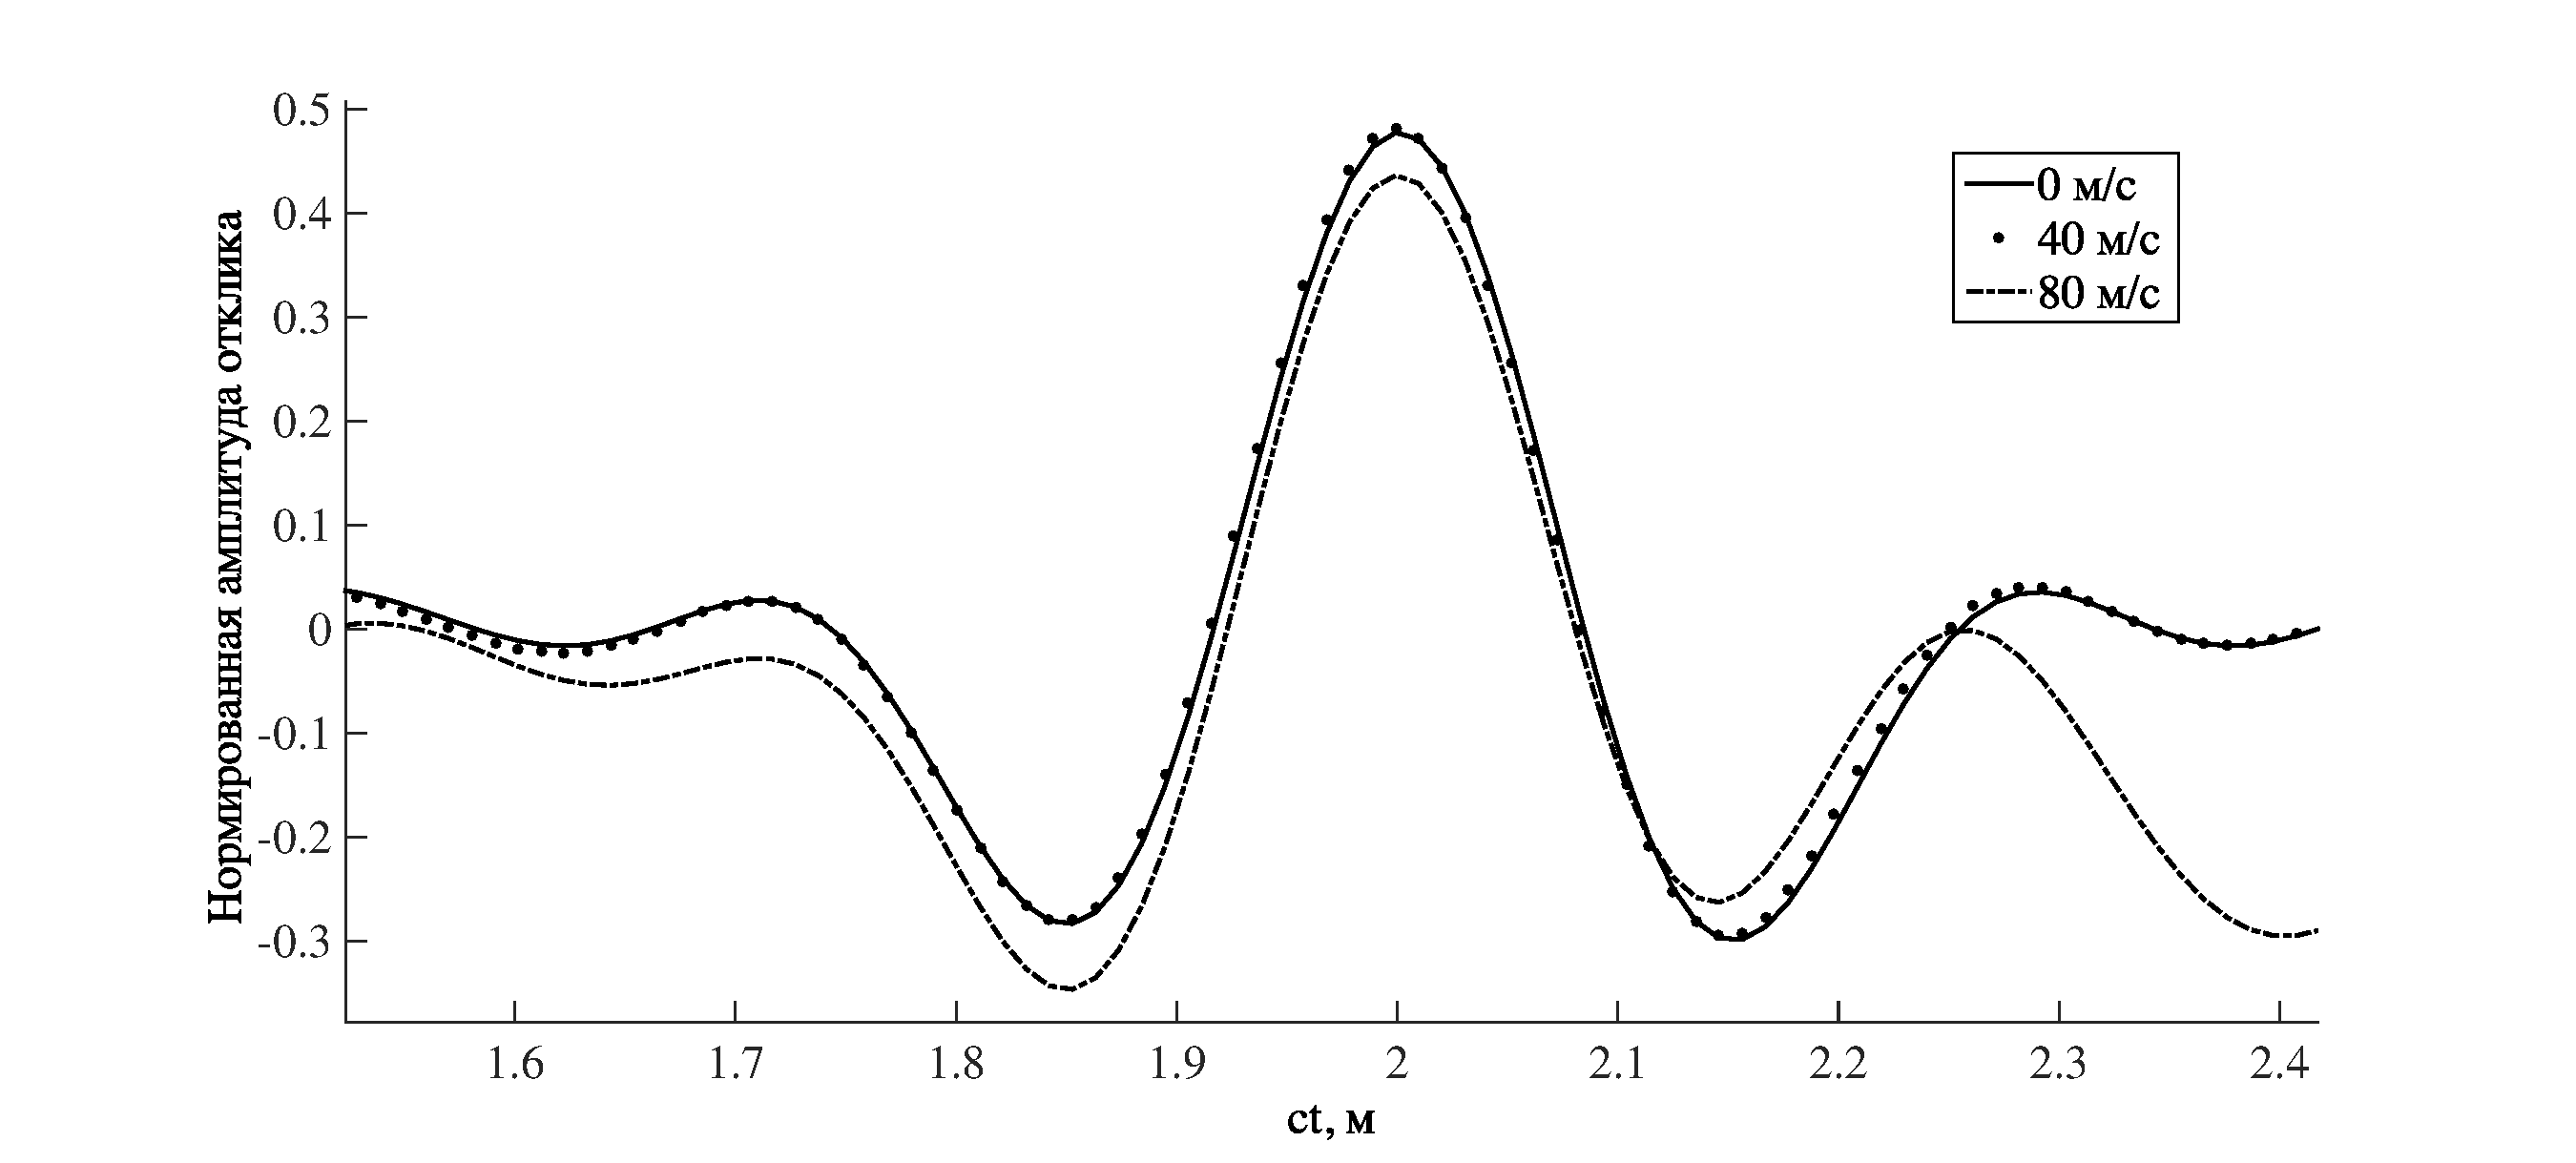
\includegraphics [scale=0.4] {ris2_8}
	\caption{Отклики на микрофоне 2 в случае, когда акустическая трасса перпендикулярна оси потока.}
	\label{img:ris2_8}
\end{figure}

\begin{figure}[ht]
	\centering
	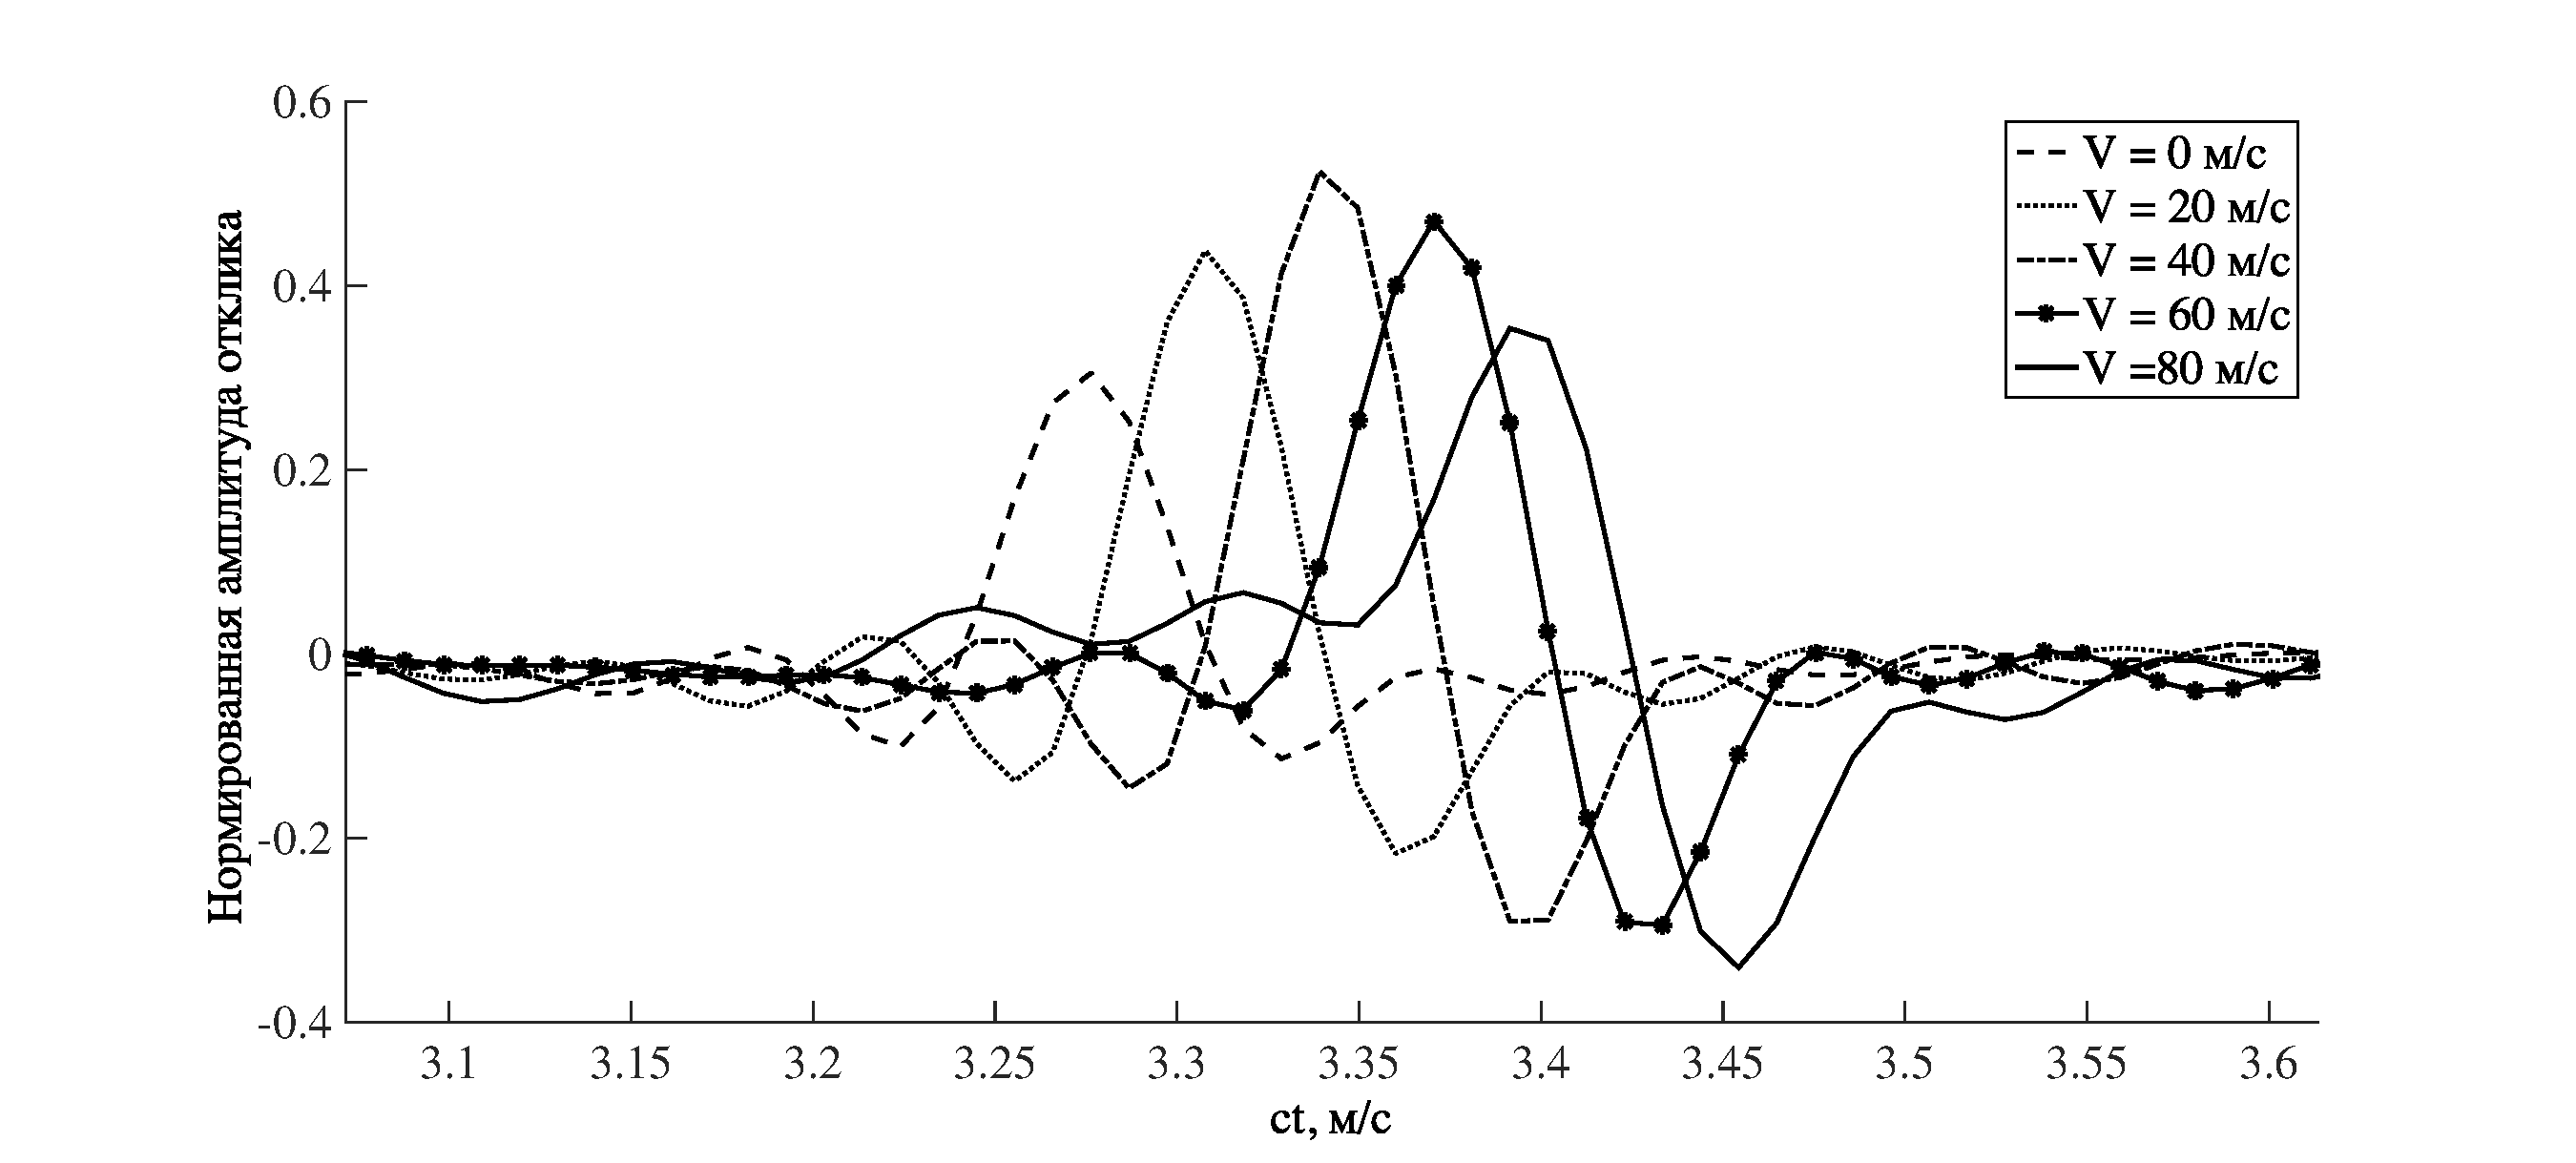
\includegraphics [scale=0.4] {ris2_9}
	\caption{Отклики на микрофоне 2 в случае, когда акустическая трасса неперпендикулярна оси потока.}
	\label{img:ris2_9}
\end{figure}


Из представленных результатов следует, что влияние потока в случае перпендикулярной трассы распространения незначительно. Отсутствие сноса сигнала и фокусировки объясняется тем фактом, что проекция луча на поток ($z$-компонента волнового вектора) в данном случае равна нулю. В случае неперпендикулярной трассы распространения, увеличение средней скорости потока приводит к увеличению задержки сигнала. Кроме того, для потоков $0, 20$ и $40$ м/c наблюдается рост амплитуды с ростом скорости потока. Наиболее вероятная причина этого роста – фокусировка сигнала. Также наблюдается падение амплитуды на скоростях $60$ м/с и $80$ м/с.

Моделирование уравнений ~\eqref{eq:2_7}, ~\eqref{eq:2_8} для координат микрофона 2 для случая неперпендикулярной трассы распространения, дает следующие значения времени задержки ~\eqref{tabular:zaderzhki}. Данные оценки неплохо согласуются с экспериментом.


\begin{table}
	\label{tabular:zaderzhki}
	\begin{center}
		\begin{tabular}{|l|l|l|l|l|l|}
			\hline
			 Поток        & Расчет         & Эксперимент    \\ \hline
			 $V = 0$  м/с & $ct = 3.280$ м & $ct = 3.280$ м \\ \hline
			 $V = 20$ м/с & $ct = 3.310$ м & $ct = 3.312$ м \\ \hline
			 $V = 40$ м/с & $ct = 3.339$ м & $ct = 3.343$ м \\ \hline			
			 $V = 60$ м/с & $ct = 3.366$ м & $ct = 3.375$ м \\ \hline			
			 $V = 80$ м/с & $ct = 3.394$ м & $ct = 3.395$ м \\ \hline
		\end{tabular}
	\end{center}
	\caption{Задержки сигналов, вычисленные с помощью ~\eqref{eq:2_7}, ~\eqref{eq:2_8} в сравнении с результатами эксперимента}
\end{table}	

На (Рис. \ref{img:ris2_10}) приводятся результаты численного моделирования сигналов методом конечных разностей для потока, скорость  струи в котором рассчитывалась с помощью ~\eqref{eq:2_10} и ~\eqref{eq:2_11}. Отметим, что результаты численного моделирования фильтруются в диапазоне $500-2000$ Гц в соответствии с пространственным разрешением сетки.

\begin{figure}[ht]
	\centering
	\includegraphics [scale=0.7] {ris2_10}
	\caption{Результат моделирования сигнала на микрофоне 2.}
	\label{img:ris2_10}
\end{figure}


Для наглядности на Рис. \ref{img:ris2_11}, Рис. \ref{img:ris2_12} совместно приведены результаты  численного моделирования и эксперимента для скоростей потока $20$ и $60$ м/с. Кроме струи ''реалистичной формы'', скорость которой рассчитывалась по формулам ~\eqref{eq:2_10} и ~\eqref{eq:2_11}, также представлены результаты моделирования для потока цилиндрической формы с постоянной по сечению скоростью.

\begin{figure}[ht]
	\centering
	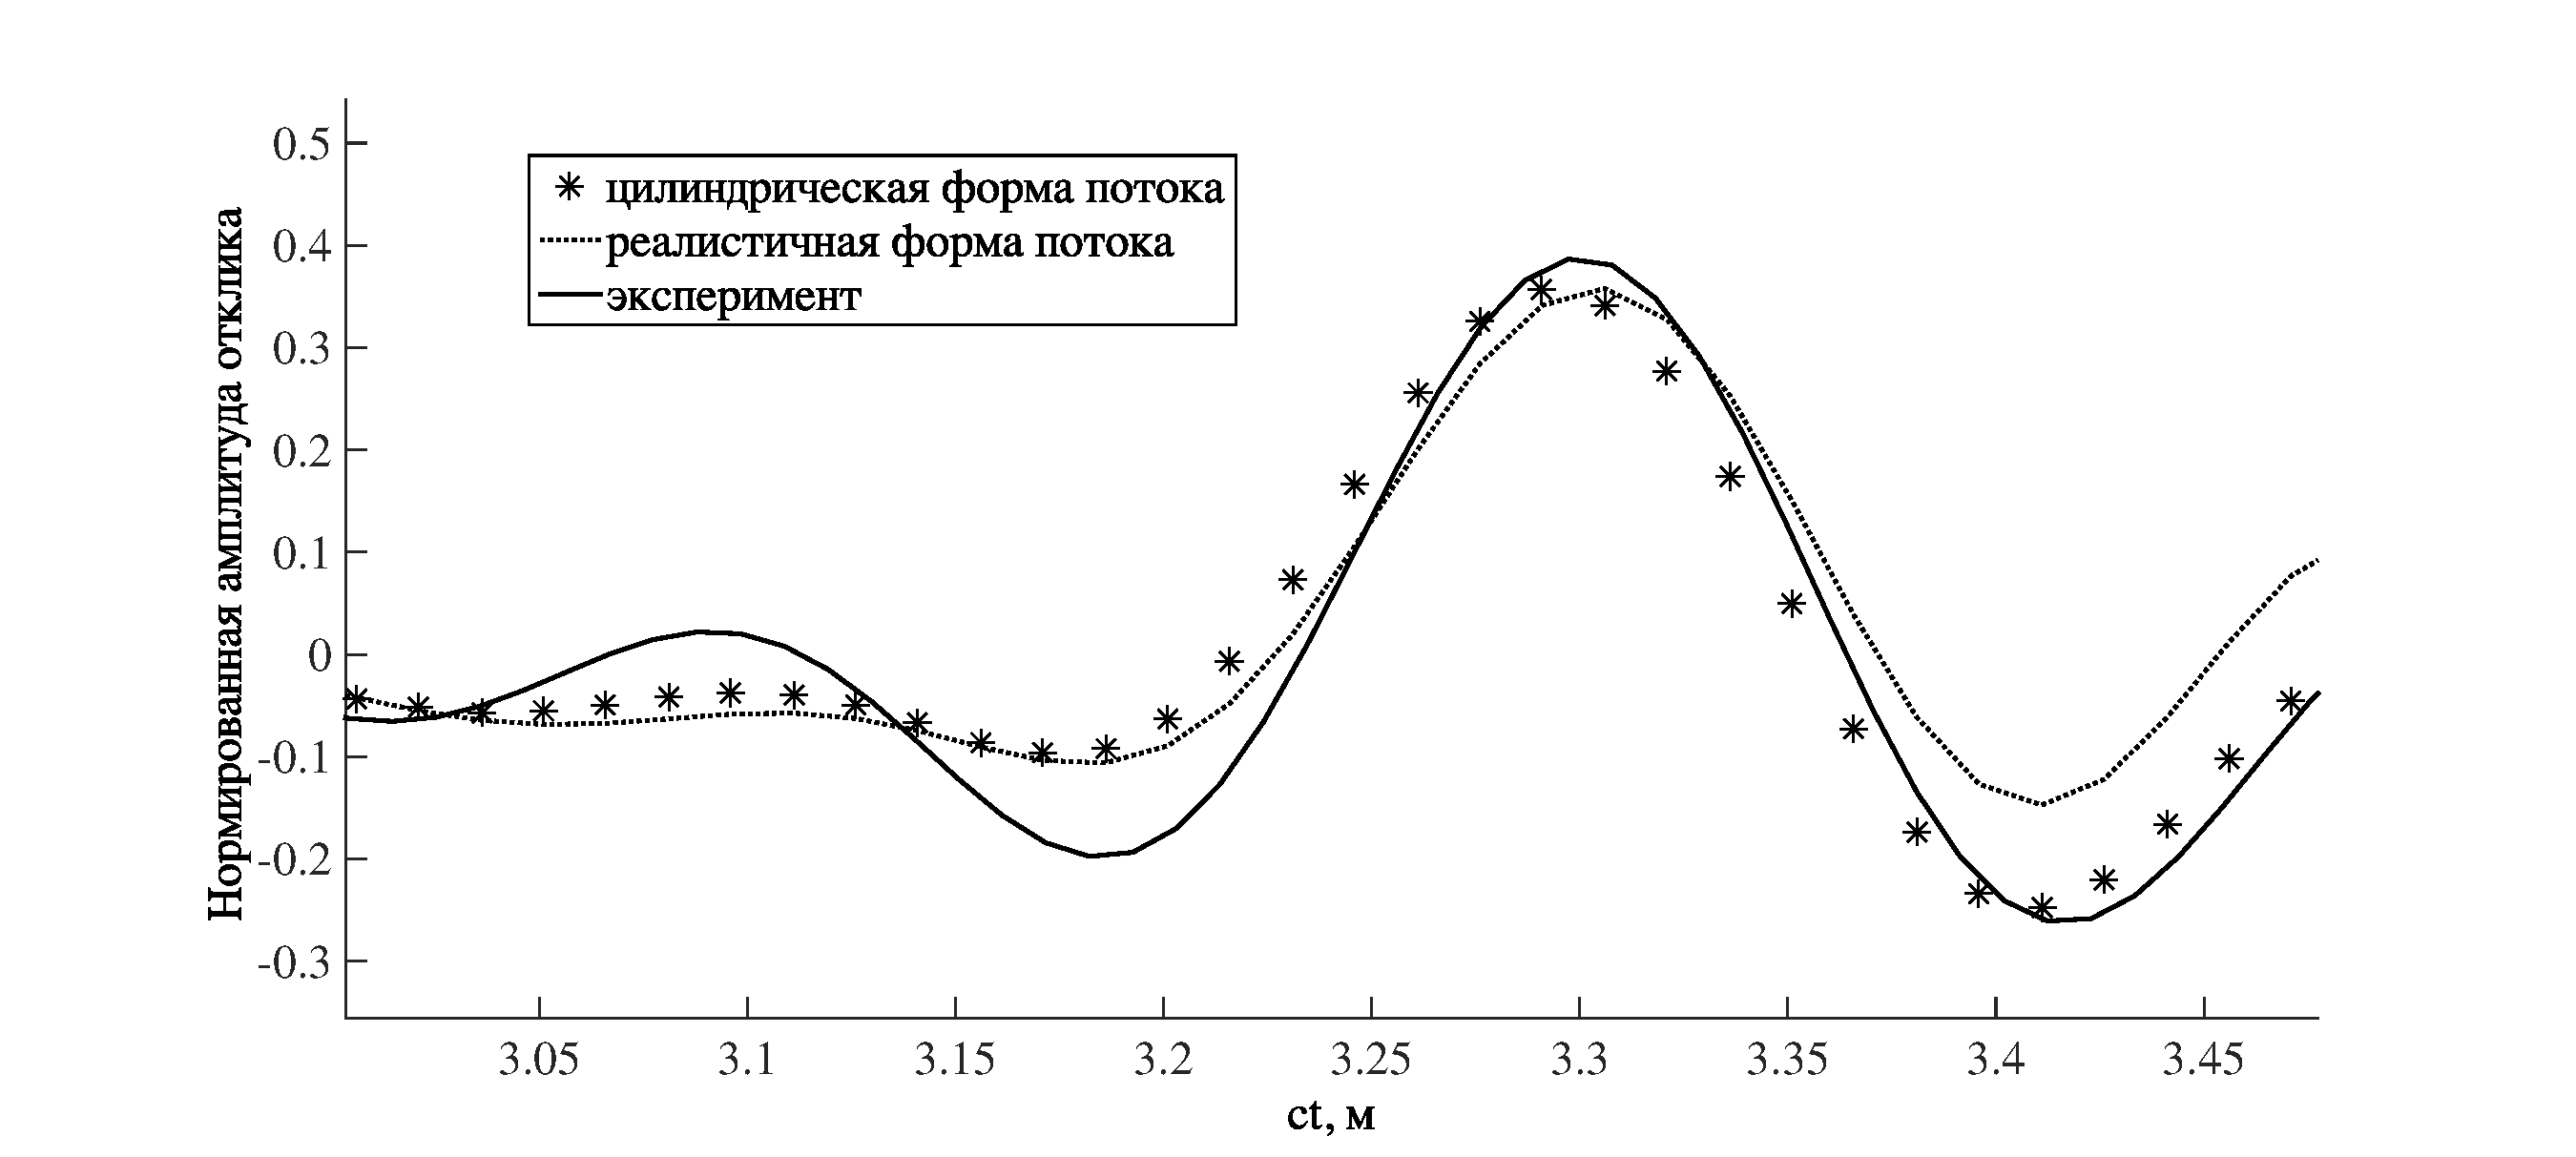
\includegraphics [scale=0.4] {ris2_11}
	\caption{Сравнение моделирования и эксперимента для микрофона 2, V = 20 м/c.}
	\label{img:ris2_11}
\end{figure}

\begin{figure}[ht]
	\centering
	\includegraphics [scale=0.6] {ris2_12}
	\caption{Сравнение моделирования и эксперимента для микрофона 2, V = 60 м/c.}
	\label{img:ris2_12}
\end{figure}


Как видно из графиков, теоретические результаты неплохо согласуются с экспериментальными данными. Также стоит отметить, что моделирование не описывает падение амплитуды сигнала на скоростях $60$ и $80$ м/с. Это косвенно свидетельствует о том, что падение амплитуды обусловлено флуктуациями в потоке, которые здесь не учитываются.

Сигналы на микрофонах 1 и 3 (выше и ниже микрофона 2, см. Рис. \ref{img:ris2_1}) слабо отличаются от сигналов на микрофоне 2. На этих микрофонах снос выражен слабее, а фокусировка приводит не к усилению, а ослаблению амплитуды.

\section{Шумы и время накопления}
	
Стоит отметить, что "сырой" сигнал на приемном микрофоне сильно зашумлен, особенно при большой скорости потока. Использование MLS техники в данном случае может рассматриваться как эффективная противошумовая мера. А именно, квазишумовые сигналы до корреляционной обработки выглядят, как показано на (Рис. \ref{img:ris2_13}, \ref{img:ris2_14}). Полезный сигнал составляет примерно $0.1$ Па, он теряется на фоне шумов уже при скорости потока $20$ м/c (шум на микрофоне составляет 1 Па), и совсем теряется при скорости потока $80$ м/c (шум составляет 10 Па). Корреляционная обработка позволяет выделить импульсный отклик весьма хорошо до $60$ м/c (Рис. \ref{img:ris2_13}).


\begin{figure}[ht]
	\centering
	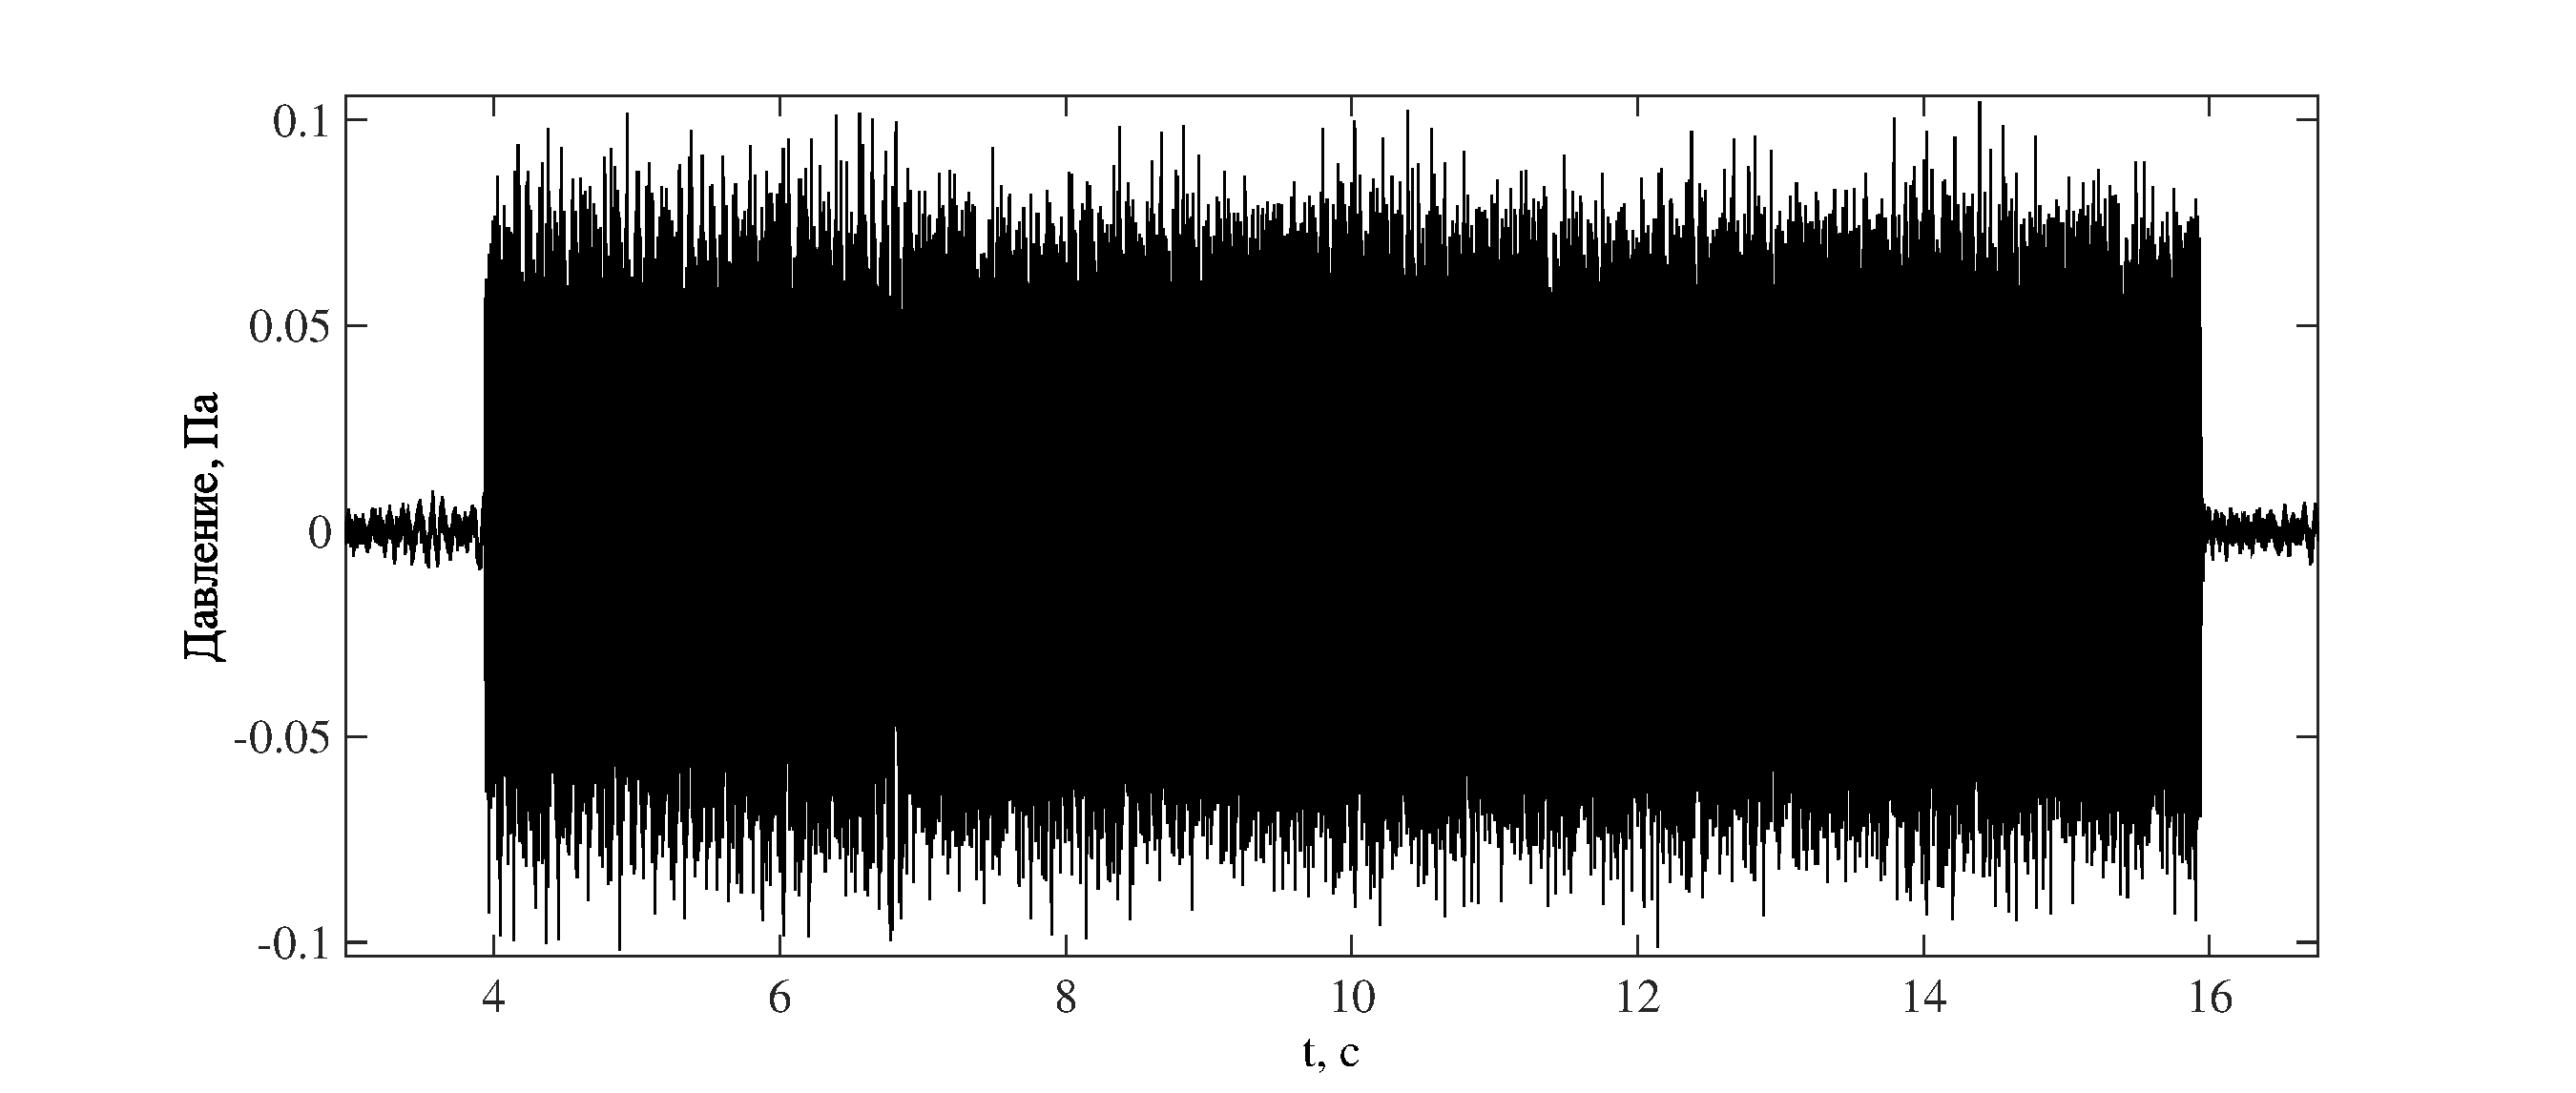
\includegraphics [scale=0.4] {ris2_13}
	\caption{Сигнал до обработки при скорости потока V = 0 м/с.}
	\label{img:ris2_13}
\end{figure}

\begin{figure}[ht]
	\centering
	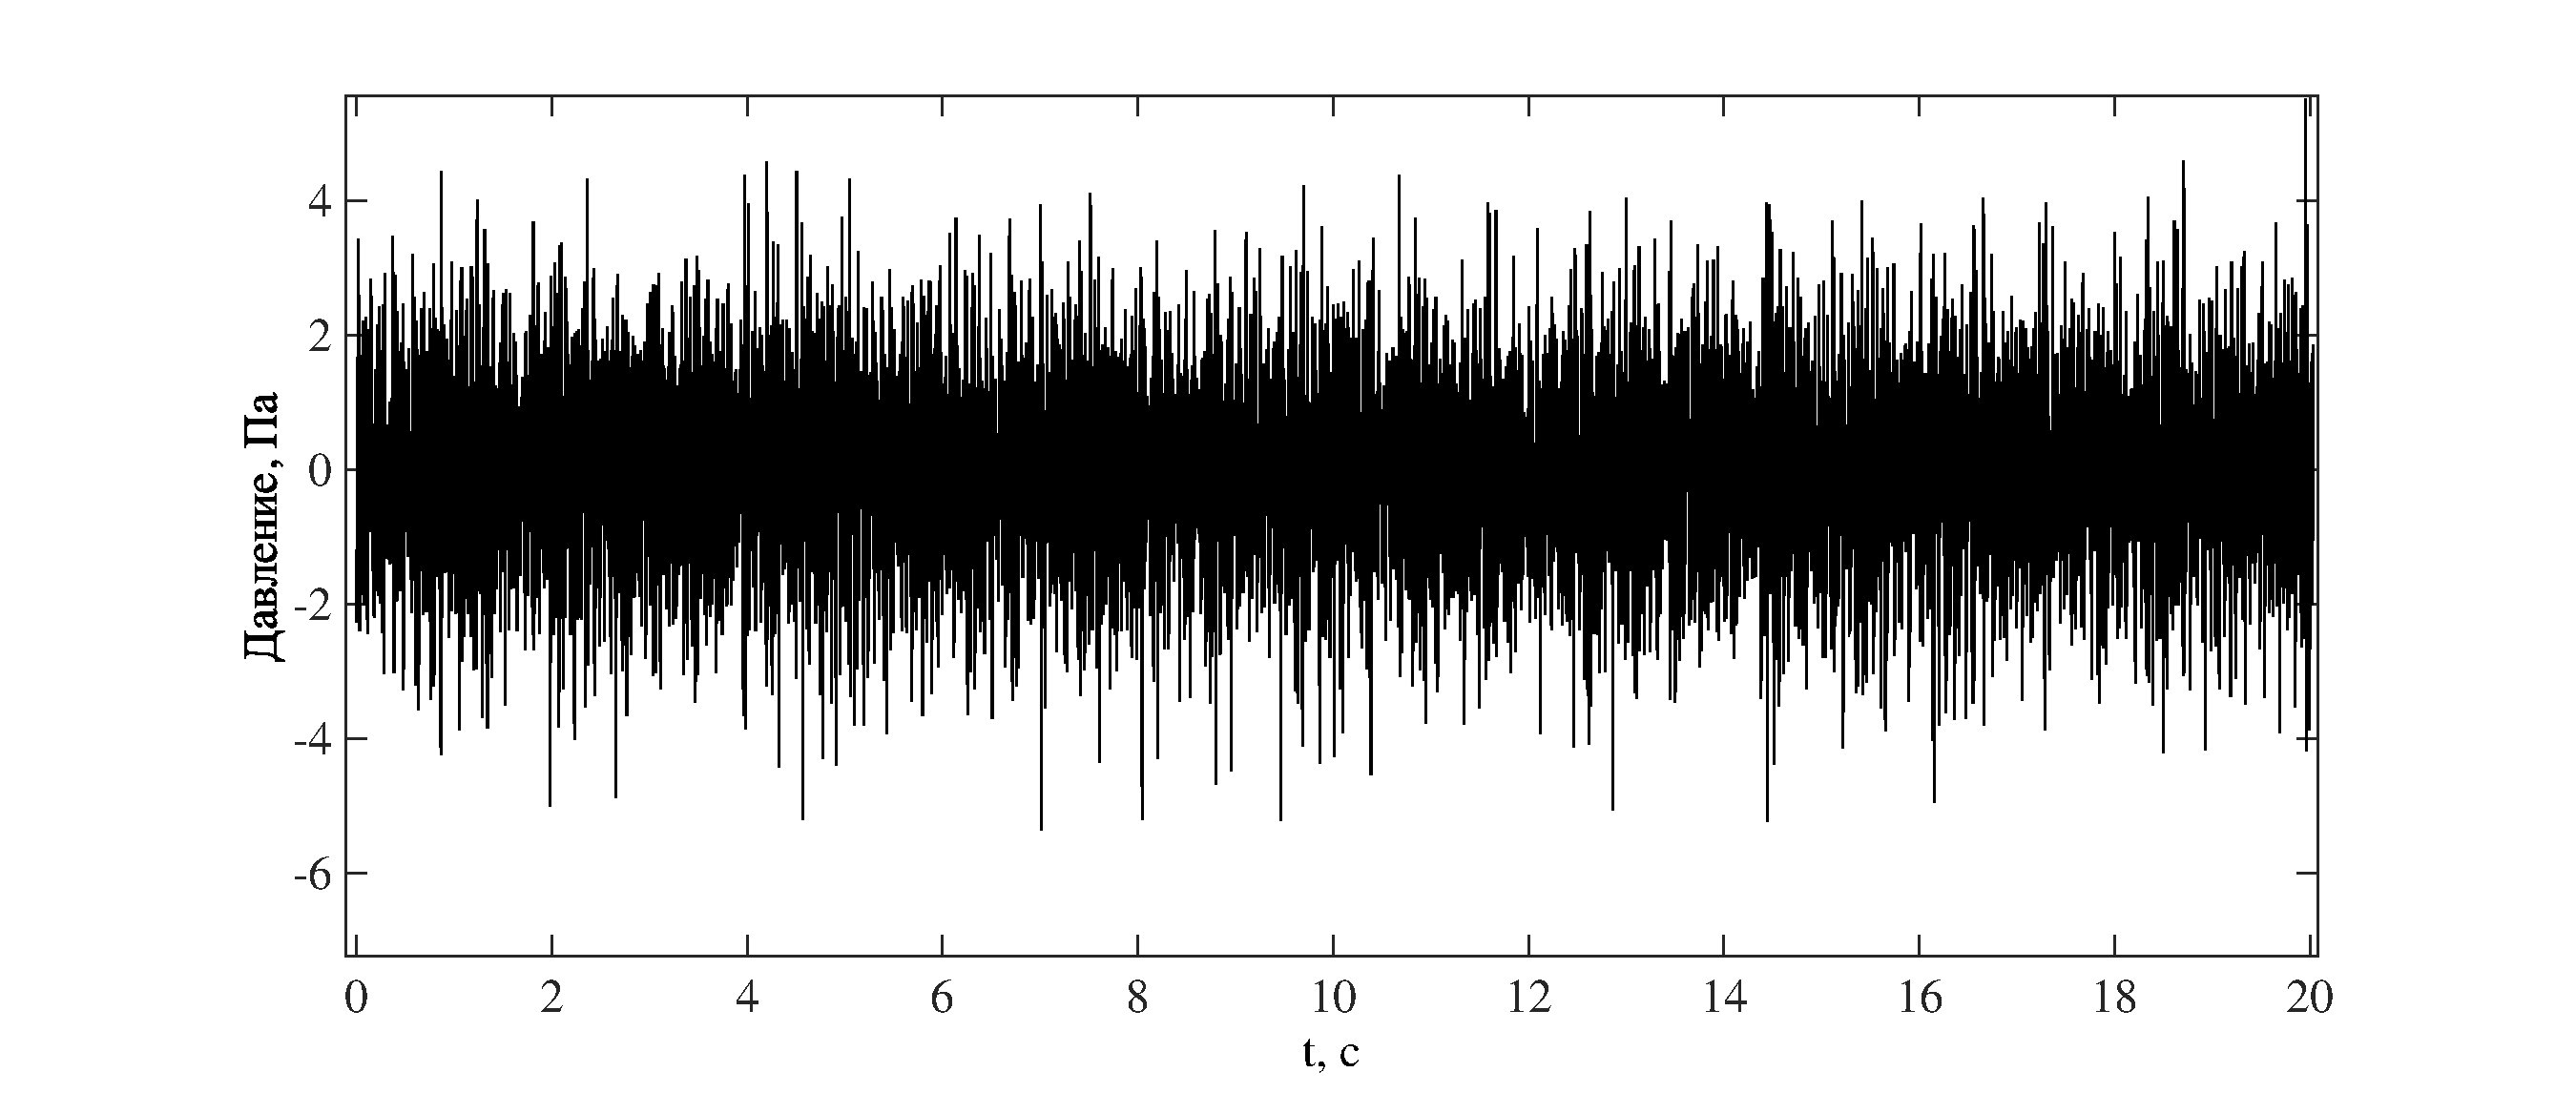
\includegraphics [scale=0.4] {ris2_14}
	\caption{Сигнал до обработки при скорости потока V = 60 м/с.}
	\label{img:ris2_14}
\end{figure}

\begin{figure}[ht]
	\centering
	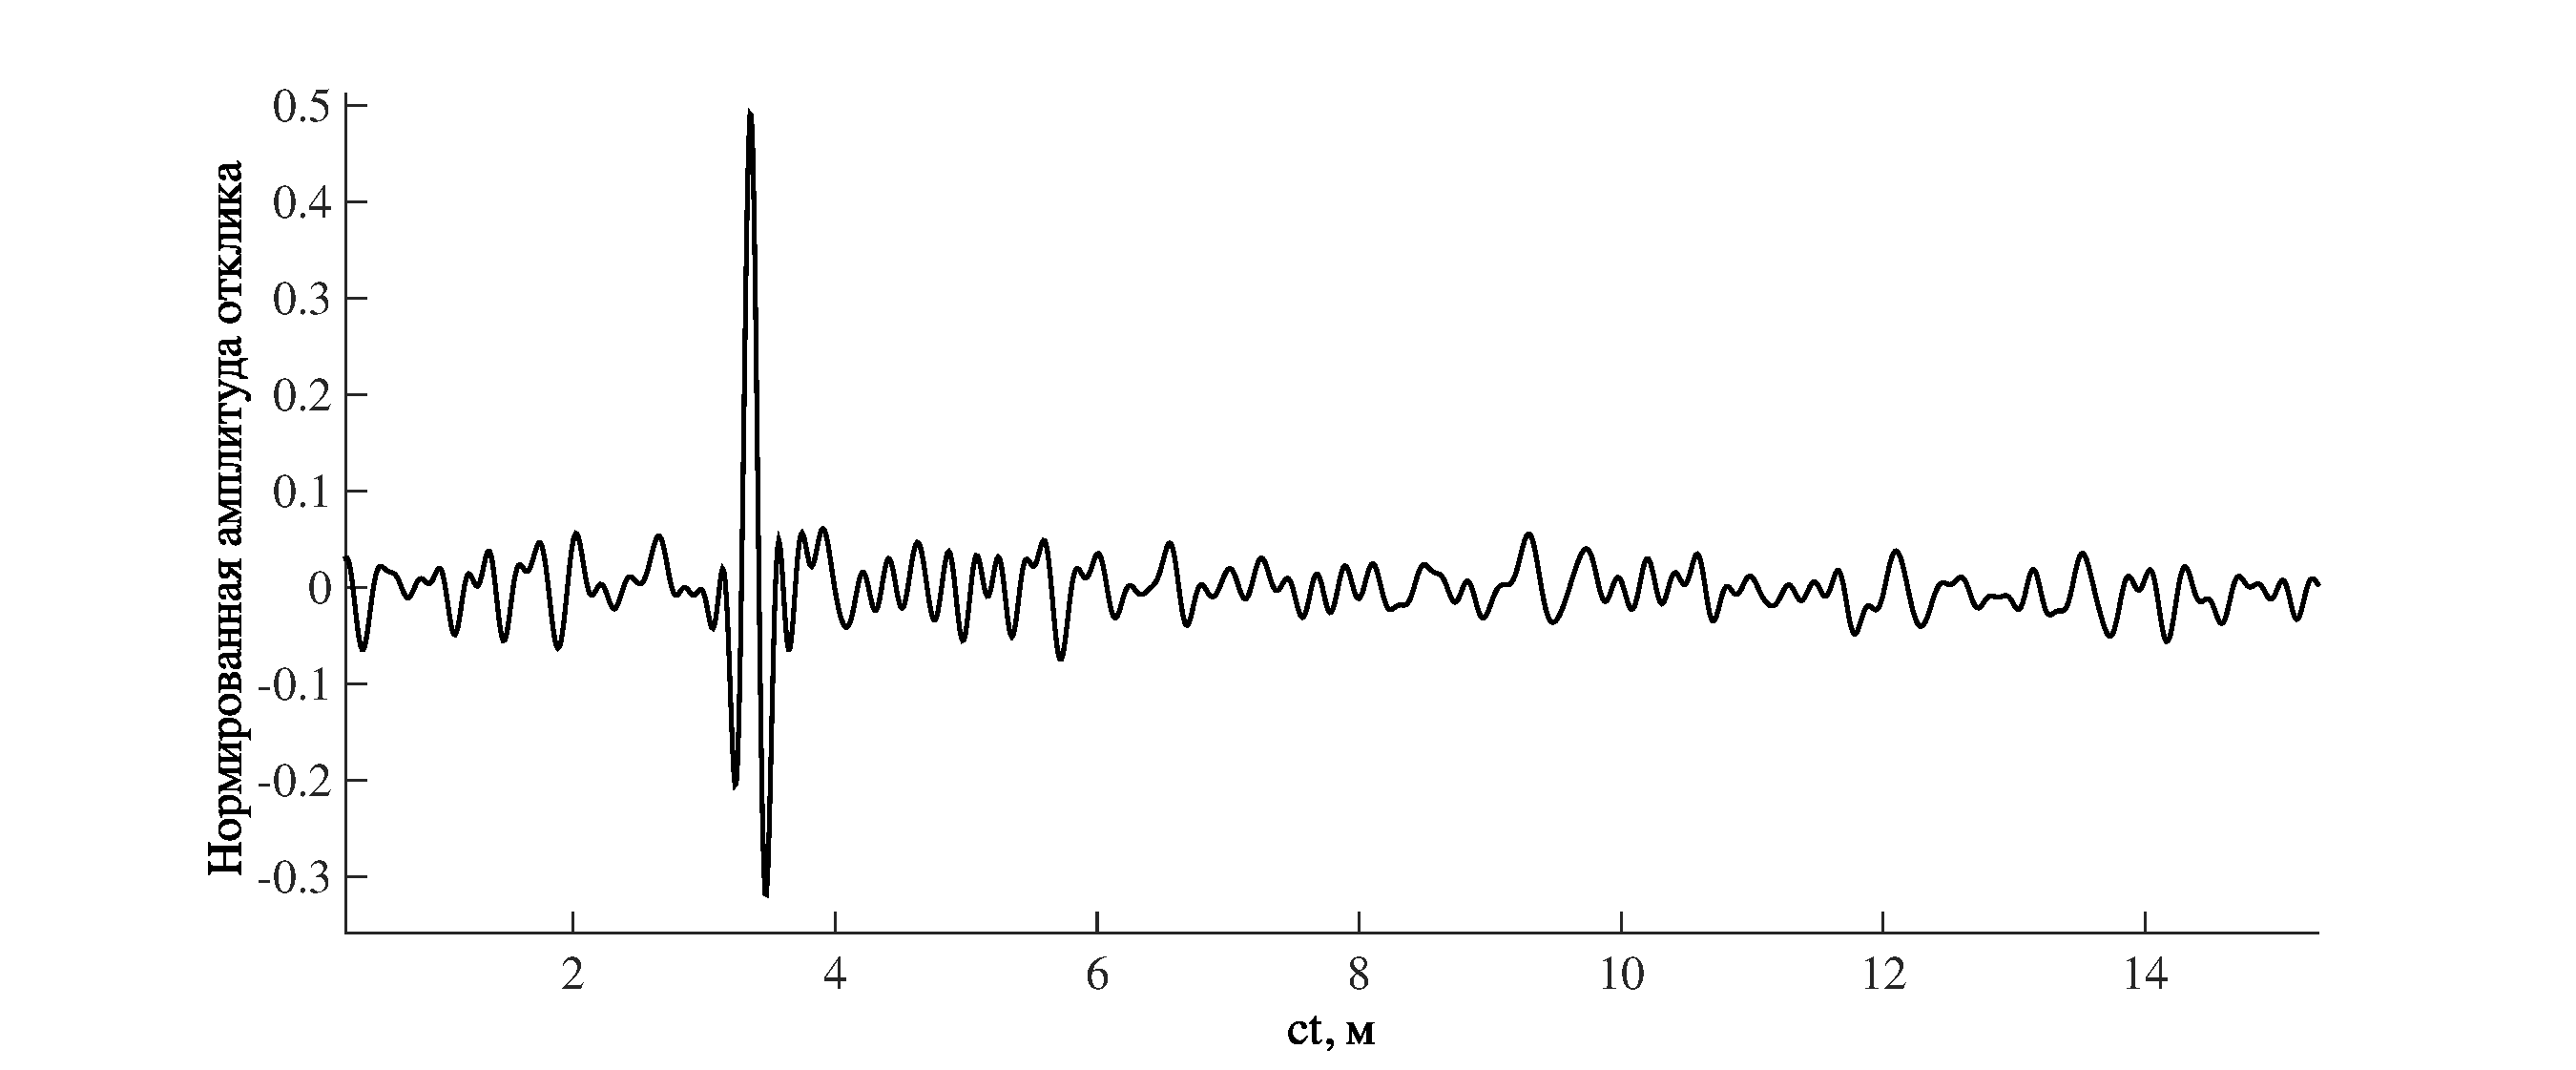
\includegraphics [scale=0.4] {ris2_15}
	\caption{Восстановленный импульсный отклик при скорости потока V = 60 м/с.}
	\label{img:ris2_15}
\end{figure}

Дальнейшее снижение шума возможно за счет увеличения времени накопления сигнала. Был проведен эксперимент по увеличению времени накопления в 3 раза. При этом средний квадрат шума снижался в 3 раза в полном соответствии с теоретическими представлениями. При работе в сильных потоках авторы предлагают увеличивать время накопления еще существеннее.

\section{Заключение}
В данной работе представлены результаты проведения прямого дифракционного эксперимента в присутствии воздушной струи. Проверялась возможность проведения измерений с использованием MLS-техники на фоне струи, создающей значительный шум. В рамках данного подхода удалось восстановить импульсный отклик, а также пронаблюдать основные эффекты, оказываемые потоком на звук: фокусировку и снос сигнала. Кроме того, был произведен теоретический расчет этих эффектов в предположении небольших чисел Маха и двух различных форм потока: цилиндрической и реалистичной, основанной на данных. Результаты расчета показали хорошее согласование с экспериментом.


\chapter{Дифракция на вытянутом теле вращения с импедансными границами. Метод граничного интегрального параболического уравнения}

В данной главе изучается задача дифракции на вытянутом теле вращения с импедансными граничными условиями. Рассматривается случай приосевого падения высокочастотной волны. Дифракционный процесс описывается с помощью метода параболического уравнения. С помощью теоремы Грина выводится граничное интегральное уравнения типа Вольтерра. Для задачи дифракции на тонком конусе с постоянным импедансом строится итерационное численное решение. Также, численные результаты сравниваются c результатами прямого дифракционного акустического эксперимента, выполненного с использованием метода M-последовательности

\section{Введение}

В этой главе рассматривается задача дифракции на вытянутом теле вращения. Иными словами, предполагается, что продольные размеры тела значительно превышают его поперечные размеры. Поле на поверхности удовлетворяет импедансным граничным условиям. Рассматривается случай приосевого падения. Также предполагается, что длины волн значительно меньше продольных размеров препятствия. При таких предположениях дифракционная задача значительно упрощается и может быть решена в рамках метода параболического уравнения.

Задачи дифракции на вытянутых телах привлекают значительное внимание исследователей. В частности, хорошо изучен случай идеальных граничных условий \cite{Andronov2011, Andronov2012, Andronov2012_2, Kirpichnikova2013, Popov2014, Engineer1998, Smyshlyaev1990, Felsen1957}. Этот случай также рассматривался авторами \cite{Shanin2011, Shanin2017}. Подробный обзор существующих методов может быть найден в \cite{Shanin2017}. К сожалению, задачи дифракции на телах вращения с импедансными граничными условиями практически не изучены. Авторам известны лишь работы, посвященные импедансному конусу \cite{Lyalinov2003, Bernard2004, Antipov2003}. В данных работах с помощью интегрального представления Конторовича-Лебедева задачу удается свести интегральному уравнению типа Фредгольма. Для случая тонкого конуса строится диаграмма направленности. В \cite{Lyalinov2009} исследовано дальнее поле вблизи поверхности конуса.

Настоящая работа является обобщением результатов, полученных в \cite{Shanin2017}, на случай импедансных граничных условий. А именно, выводится граничное интегральное уравнение в параболической постановке. Полученное уравнение относится к классу Вольтерра, что позволяет его решить с помощью метода итераций.

В работе выводятся интегральные уравнения двух типов. Уравнение первого типа, более общее, является двумерным и имеет ядро, зависящее от четырех переменных: двух координат источника и двух координат приемника на поверхности препятствия. Данное уравнение формулируется для произвольного вытянутого тела. Путем учета угловой симметрии выводится ряд одномерных уравнений для угловых мод. Эти уравнения, соответственно, справедливы только для тел вращения. При осевом падении остается только уравнение для нулевой моды, которое решается методом итераций для задачи дифракции на конусе с постоянным импедансом.

Кроме того, полученные численные и аналитические результаты сравниваются с результатами прямого акустического дифракционного эксперимента, выполненного с применением метода M-последовательности. Сравнение проводится для случая идеальных граничных условий Неймана.

\section{Постановка задачи}

\subsection{Постановка задачи для уравнения Гельмгольца}

Рассмотрим трехмерное пространство, описываемое цилиндрическими координатами $(x, r, \varphi)$. Будем считать, что $x$ — продольная координата в том смысле, что все волновые процессы происходят под малым углом к оси $x$. Пусть везде вне тела выполняется уравнение Гельмгольца:

\begin{eqnarray}
\label{eq:helmholtz}
\left(\frac{\partial^2}{\partial x^2} + \Delta_\perp + k^2\right) \tilde{u}(x, r, \varphi) = 0, \\
\Delta_\perp = \frac{1}{r} \frac{\partial}{\partial r} r \frac{\partial}{\partial r} + \frac{1}{r^2} \frac{\partial}{\partial \varphi}
\end{eqnarray}

Временная зависимость имеет форму $\exp(-i\omega t)$ и далее не выписывается. Тело вращения занимает симметричную относительно оси $x$  область $r < f(x)$. Будем обозначать поверхность тела символом $\Gamma$. Тело может быть как компактным $(X_1 \leq x \leq X_2)$, так и полубесконечным $(x \geq X_1)$. Примером тела вращения является конус:
\begin{equation}
\label{eq:straightline}
r = f(x) = \alpha x, x\geq 0.
\end{equation}

Падающая волна имеет вид:
\begin{equation}
\label{eq:inc_small_angle}
\tilde{u}^{\text{in}} = \exp\{ik(x\cos \theta + r \cos \varphi \sin \theta)\},
\end{equation}
где угол падения $\theta$ предполагается малым. 

Полное поле $\tilde{u}$ представляется в следующем виде:

\begin{equation}
\tilde{u} = \tilde{u}^{\text{in}} + \tilde{u} ^ {\text{sc}}.
\end{equation}

Здесь $\tilde{u}^{\text{sc}}$ — рассеянное поле, удовлетворяющее условиям излучения. Условия излучения формулируются в виде принципа предельного поглощения. А именно, предполагается, что волновое число $k$ имеет малую положительную мнимую часть. Следовательно, рассеянное поле затухает при $|x| \rightarrow \infty$ или $|r| \rightarrow \infty$.

На поверхности тела должны выполняться импедансные граничные условия:

\begin{equation}
\label{eq:imp_usl}
\frac{\partial \tilde{u}}{\partial \textbf{n}} = \eta \tilde{u},
\end{equation}
где $\eta$ - импеданс, $\textbf{n}$ - внешняя нормаль к поверхности тела. На импеданс накладывается условие неизлучения энергии

\begin{equation}
\label{eq:neizl}
\text{Im}\left[\eta\right] \leq 0.
\end{equation}

Если на поверхности тела имеются конические точки (такие, как вершина конуса), то в них должны удовлетворяться условия Мейкснера, заключающиеся в интегрируемости «энергии» $|\nabla \tilde{u}|^2 + |\tilde{u}|^2$ вблизи конической точки.

\subsection{Постановка задачи для параболического уравнения}

Предполагается, что тело вращения вытянуто в том смысле, в котором это понятие было введено в \cite{Shanin2017}. А именно, предполагается, что дифракционный процесс носит приосевой характер, т. е. выполнены следующие условия:

\begin{itemize}
	\item Угол падения мал: $\theta \ll 1$.
	\item Наклон поверхности меняется плавно: $\dot{f} \ll 1$. Здесь $\dot{f}$ - производная $df/dx$.
	\item Угол дифракции мал: $(\ddot{f}/k)^{1/3} \ll 1$. Здесь $\ddot{f}$ - прозводная $d^2 f/ dx^2$.
\end{itemize}

Поясним последнее условие. Продольный размер зоны Френеля определяется выражением \cite{Fok1970}:

\begin{equation}
\label{eq:long_fresnel}
\Delta x = \left(\ddot{f}\right)^{-2/3} k^{-1/3}.
\end{equation}

Угол дифракции может быть оценен как изменение наклона поверхности на $\Delta x$, т.е. как $\Delta x \ddot{f} = \left(\ddot{f}/k\right)^{1/3}$.

В соответствии с методом параболического уравнения, представим полное поле в виде

\begin{equation}
\label{eq:inc_wave}
\tilde{u}(x, r, \varphi) = e^{ikx} u(x, r, \varphi),
\end{equation}
где $u(x,r,\varphi)$  является медленной функцией $x$ по сравнению с экспоненциальным множителем. Подставляя ~\eqref{eq:inc_wave} в ~\eqref{eq:helmholtz} и пренебрегая членом с второй производной по $x$, получаем параболическое уравнение теории дифракции (ПУТД):

\begin{equation}
\label{eq:putd}
\left(\frac{\partial}{\partial x} + \frac{1}{2ik} \Delta_\perp\right) u = 0.
\end{equation}

Падающая волна ~\eqref{eq:inc_small_angle} в параболическом приближении принимает вид

\begin{equation}
\label{eq:inc_wave2}
u^{\text{in}} (x, r, \varphi) = \exp\{ ik \left(\theta r \cos \varphi  - x\theta^2 / 2 \right) \},
\end{equation}
где учтено, что $\cos \theta \approx 1 - \theta^2/2$, $\sin \theta \approx \theta$. Легко проверить, что ~\eqref{eq:inc_wave2} удовлетворяет ~\eqref{eq:putd}. В случае осевого падения $\theta = 0$ имеем

\begin{equation}
u^{\text{in}} = 1.
\end{equation}

Импедансные граничные условия ~\eqref{eq:imp_usl} переходят в

\begin{equation}
\label{eq:imp_cond2}
N\left[u\right](x, f(x), \varphi) = \eta u, \quad N \equiv \frac{\partial}{\partial r} - ik\dot{f}.
\end{equation}

Переход от $\partial/\partial n$ к $N$ подробно обсуждается в \cite{Shanin2017}. А именно, непосредственно вычисляя производную от ~\eqref{eq:inc_wave}, и пренебрегая членами порядка $\left(\dot{f}\right)^2$, получим ~\eqref{eq:imp_cond2}.

Как известно, наличие импедансных граничных условий может приводить к появлению поверхностных волн. Если их скорость существенно меньше скорости волн в среде, параболическое приближение не будет справедливым. Потребуем выполнения следующего условия

\begin{equation}
\label{eq:potrebuem_sled}
\eta/k \ll 1.
\end{equation}

Тогда скорость распространения поверхностных волн будет близка к скорости звука \cite{Korolkov2016}, и, следовательно, они будут хорошо описываться параболическим приближением. Также предполагается выполнение условия неизлучения энергии ~\eqref{eq:neizl}.


Постановка задачи для ПУТД должна быть дополнена начальным условием
\begin{equation}
u^{\text{sc}} = 0, \quad \text{при} \quad x<X_1,
\end{equation}
отражающим тот факт, что ПУТД описывает только волны, распространяющиеся в положительном направлении.

Кроме того, должны выполняться условия излучения, накладываемые в виде принципа предельного поглощения.

Наконец, требуется выполнение условий Мейкснера. А именно, вблизи конической точки требуется локальная интегрируемость следующего выражения \cite{Shanin2017}:

\begin{equation}
|\Delta_\perp u|^2 + |u|^2.
\end{equation}

\section{Вывод граничного интегрального уравнения}

\subsection{Теорема Грина для параболического уравнения}
Введем векторные обозначения для точек пространства $\textbf{r} = (x, r, \varphi)$. Определим функцию Грина как решение неоднородного параболического уравнения с источником в точке $\textbf{r}_s = (x_s, r_s, \varphi_s)$:

\begin{equation}
\label{eq:neodn_parabol}
\left(\frac{\partial}{\partial x} + \frac{1}{2ik} \Delta_\perp \right) g(\mathbf{r}, \mathbf{r_s}) = \delta(\mathbf{r}, \mathbf{r_s}),
\end{equation}
где оператор в левой части действует на компоненты вектора $\textbf{r}$, а $\delta$ — дельта-функция Дирака. Решение уравнения должно удовлетворять начальному условию, то есть должно обращаться в ноль при $x < x_s$. При помощи непосредственной подстановки в ~\eqref{eq:neodn_parabol} можно убедиться, что функция Грина при $x>x_s$ имеет следующий вид:

\begin{equation}
g(\textbf{r}, \mathbf{r_s}) = \frac{k}{2 \pi i (x-x_s)} \exp \{\frac{ik}{2} \frac{(\Delta r)^2}{x-x_s} \},
\end{equation}
где $\Delta r$ - расстояние между проекциями векторов в поперечной плоскости:

\begin{equation}
(\Delta r)^2 = r^2 + r_s^2 - 2r r_s \cos(\varphi - \varphi_s).
\end{equation}

Сформулируем теорему Грина для параболического уравнения. Пусть $\Omega$ - конечная связная область с гладкой границей $\partial \Omega$  и внешней нормалью $\textbf{n}$. Рассмотрим пару неоднородных параболических уравнений

\begin{equation}
\label{eq:eq18}
\left(\frac{\partial}{\partial x} + \frac{1}{2ik} \Delta_\perp\right) v(x, r, \varphi) = q(x, r, \varphi),
\end{equation}

\begin{equation}
\left(-\frac{\partial}{\partial x} + \frac{1}{2ik} \Delta_\perp\right) w(x, r, \varphi) = h(x, r, \varphi)
\end{equation}
для некоторых $v, q, w, h$. Отметим, что второе уравнение является комплексно сопряженным к первому, то есть описывает распространение волн в отрицательном направлении. 

Введем векторные функции:

\begin{equation}
\textbf{v}(x,y,z) = \left( ikv, \frac{\partial v}{\partial r}, \frac{1}{r} \frac{\partial v}{\partial \varphi} \right), \quad \mathbf{w}(x,y,z) = \left( -ikw, \frac{\partial w}{\partial r}, \frac{1}{r} \frac{\partial w}{\partial \varphi} \right)
\end{equation}

Наконец, сформулируем теорему Грина \cite{Shanin2017}:

\begin{equation}
\int_{\partial \Omega} [ (\mathbf{v \dot n}) w - (\mathbf{w \dot n}) v  ] dS = 2ik \int_{\Omega} [qw - hv ] dV.
\end{equation}

\subsection{Граничное интегральное уравнения для полного поля}

\begin{figure}[ht]
	\centering
	\includegraphics [scale=0.5] {ris3_1}
	\caption{Сечение области для теоремы Грина.}
	\label{img:ris3_1}
\end{figure}

Применим теорему Грина к области $\Omega$, сечение которой изображено на Рис. \ref{img:ris3_1}. Область ограничена плоскостью $x = X$, где $X < X_1$, плоскостью $x = x_*$ для некоторого $x_*$, цилиндром $r = R$, где $R \rightarrow \infty$, и поверхностью тела вращения $\Gamma$. Область $\Omega$ обладает осевой симметрией относительно оси $x$. В качестве $v$ подставим в ~\eqref{eq:eq18} рассеянное поле $u^{\text{sc}}$, а в качестве $w$ подставим $g(\mathbf{r_*, r})$, где 

\begin{equation}
r_* = (x_* + \varepsilon, f(x_* + \varepsilon), \varphi_*).
\end{equation}

Здесь $\varphi_*$ предполагается произвольным, $\varepsilon$ — малым (ниже рассматривается предел $\varepsilon \rightarrow 0$). Проводя выкладки, аналогичные таковым в \cite{Shanin2017}, получаем следующее интегральное уравнение:

\begin{multline}
\label{eq:u_sc}
U^{\text{sc}}(x_*, \varphi_*) = \frac{i}{k} \int_{0}^{2\pi} \int_{X_1}^{x_*} U^{\text{sc}}(x,\varphi) \{\bar{N}\left[W\right](x,\varphi) - \eta W(x, \varphi) \} f(x) dx d\varphi + \\
\frac{i}{k} \int_{0}^{2\pi} \int_{X_1}^{x_*} W(x, \varphi) \{ N \left[U^{\text{in}} \right] (x, \varphi)  - \eta U^{\text{in}}(x, \varphi) \} f(x) dx d\varphi,
\end{multline}
где были введены следующие обозначения:

\begin{eqnarray}
&\bar{N} \equiv \frac{\partial}{\partial r} - ik \frac{df}{dx}, \\
&U^{\text{sc}} (x, \varphi) \equiv u^{\text{sc}}(x, f(x), \varphi), \\
&U^{\text{in}} (x, \varphi) \equiv u^{\text{in}}(x, f(x), \varphi), \\
& W(x, \varphi) \equiv w(x, f(x), \varphi).
\end{eqnarray}

Введем обозначение для ядра уравнения ~\eqref{eq:u_sc}:

\begin{equation}
\label{eq:obosn_dlya_yadra}
K(x_*, \varphi_*, x, \varphi) \equiv \frac{i f(x)}{k} ( \bar{N} \left[W\right] (x,\varphi) - \eta W(x, \varphi) ).
\end{equation}

Уравнение ~\eqref{eq:u_sc} может быть упрощено. А именно, применяя теорему Грина к области $\Omega$ с функциями

$$v(r) = u^{\text{in}}(r), \quad w(r) = g(r_*, r),$$
получим интегральное соотношение:

\begin{multline}
\label{eq:u_in}
U^{\text{in}}(x_*, \varphi_*) = \frac{i}{k} \int_{0}^{2\pi} \int_{X_1}^{x_*} U^{\text{in}}(x,\varphi) \{\bar{N}\left[W\right](x,\varphi) - \eta W(x, \varphi) \} f(x) dx d\varphi + \\
\frac{i}{k} \int_{0}^{2\pi} \int_{X_1}^{x_*} W(x, \varphi) \{ N \left[U^{\text{in}} \right] (x, \varphi)  - \eta U^{\text{in}}(x, \varphi) \} f(x) dx d\varphi + 2 U^{\text{in}}(x_*, \varphi_*),
\end{multline}

Складывая ~\eqref{eq:u_sc} и ~\eqref{eq:u_in}, получим уравнение для полного поля $U = U^{\text{sc}} + U^{\text{in}}$  на поверхности тела:

\begin{equation}
\label{eq:main_intur}
U(x_*, \varphi_*) = \int_{0}^{2 \pi} \int_{X_1}^{x_*} K(x_*, \varphi_*, x, \varphi) U(x, \varphi) dx d\varphi + 2 U^\text{in} (x_*, \varphi_*).
\end{equation}

Ядро ~\eqref{eq:u_sc} дается следующим выражением:

\begin{equation}
\label{eq:yadro_intura}
K(x_*, \varphi_*, x, \varphi) = \frac{ikf(x)}{2 \pi} \left( \frac{1}{ik} \frac{ik\dot{f}(x) - \eta}{x_* - x}  + \frac{f(x) - f(x_*) \cos(\varphi - \varphi_*)}{(x_* - x)^2}\right) \times \exp \{ \frac{ik}{2} \frac{(f(x))^2  + (f(x_*))^2 - 2f(x_*) f(x_*) \cos(\varphi - \varphi_*) }{x_* - x} \}
\end{equation}

Уравнение ~\eqref{eq:main_intur} является уравнением Вольтерра по переменной $x$ и уравнением с разностным ядром по переменной $\varphi$.

\subsection{Граничное интегральное уравнение для угловых мод}

Воспользуемся осевой симметрией задачи. Представим падающее и полное поля на поверхности тела в виде рядов Фурье:

\begin{equation}
\label{eq:fourier_in_full}
U^{\text{in}}(x, \varphi) = \sum_{n = -\infty}^{\infty} U^{\text{in}}_n (x) e^{in \varphi}, \quad U(x,\varphi) = \sum_{n = -\infty}^{\infty} U_n(x) e^{in\varphi}.
\end{equation}
Функции $U_n$  удовлетворяют следующим интегральным уравнениям:

\begin{equation}
U_n(x_*) = \int_{X_1}^{x_*} K_n(x_*, x) U_n(x) dx + 2 U^{\text{in}} (x_*),
\end{equation}
где
\begin{equation}
K_n(x_*, x) = \int_{0}^{2 \pi} K(x_*, \varphi, x, 0) e^{-in\varphi} d\varphi.
\end{equation}

Используя ~\eqref{eq:yadro_intura}, можно получить явное выражение для $K_n(x_*, x)$:

\begin{equation}
K_n(x) = \frac{-(-i)^{n+1}}{(x_* - x)^2} \exp \{ \frac{ik}{2} \frac{r_*^2 + r^2}{x_* - x} \} \left[ \left(r + (x_* - x) \left( \frac{df}{dx} - \frac{\eta}{ik} \right) \right)J_n(\frac{k r_* r}{x_* - x}) - \frac{ir_*}{2} \left( J_{n-1}\left(\frac{kr_*r}{x_*-x}\right) - J_{n+1}\left(\frac{k r_* r}{x_*-x}\right)  \right)\right],
\end{equation}
где $r = f(x)$, $r_* = f(x_*)$, $J_n$ - функция Бесселя первого рода.
Стоит отметить, что по аналогии с \cite{Shanin2017} для конечного тела вращения может быть получено выражение для диаграммы направленности и доказана оптическая теорема.

\section{Дифракция на импедансном конусе при осевом падении}

\subsection{Граничное интегральное уравнение для конической задачи при осевом падении}

Рассмотрим конус, для которого $X_1 = 0$, т. е. вершина конуса находится в начале координат, как показано на Рис. \ref{img:ris3_2}. Профиль конуса представляет собой прямую линию ~\eqref{eq:straightline}, где $\alpha$ является тангенсом угла между осью конуса и его образующей. Предполагается, что $\alpha \ll 1$.
 
 \begin{figure}[ht]
 	\centering
 	\includegraphics [scale=0.5] {ris3_2}
 	\caption{Геометрия задачи дифракции на конусе.}
 	\label{img:ris3_2}
 \end{figure}
 
Пусть падающая волна распространяется вдоль оси $x$, то есть имеет вид ~\eqref{eq:putd}. В этом случае полное поле обладает осевой симметрией и описывается нулевой компонентой ряда ~\eqref{eq:fourier_in_full}:
$$U(x, \varphi) = U_0(x) = U(x).$$

Тогда задача сводится к одномерному интегральному уравнению:

\begin{equation}
\label{eq:big_int_eq}
U(x_*) = \int_{0}^{x_*} K_0(x_*, x) U(x) dx + 2
\end{equation}
с ядром
\begin{equation}
K_0 = \frac{ik \alpha^2 x_* x}{(x_* - x)^2} \exp \{ \frac{ik \alpha^2}{2} \frac{x_*^2 + x^2}{x_* - x} \} \times \left[  J_0\left( k \alpha^2 \frac{x x_*}{x_* - x} \right) + i J_1\left( k \alpha^2 \frac{x x_*}{x_* - x} \right) - \frac{\eta (x_* - x)}{ikx_* \alpha}J_0 \left(k \alpha^2 \frac{x x_*}{x_* - x}\right)  \right].
\end{equation}

\subsection{Случай разделяющихся переменных}

Пусть импеданс меняется обратно пропорционально $x$:

\begin{equation}
\label{eq:imp_obr_prop}
\eta = \frac{\tilde{\eta}}{x}.
\end{equation}

Тогда задача для параболического уравнения может быть решена с помощью метода разделения переменных. Перейдем в систему координат $(x, \rho, \varphi)$ с

\begin{equation}
\rho = r/x,
\end{equation}
и введем новую полевую переменную $\hat{u}$:

\begin{equation}
u(x, \rho x, \varphi) = \Xi^{-1} (x, \rho) \hat{u}(x, \rho, \varphi), \quad \Xi(x, \rho) \equiv kx \exp \{ -ikx\rho^2/2 \}.
\end{equation}

Уравнение ~\eqref{eq:putd} переходит в

\begin{equation}
\label{eq:putd_perehodit_v}
\left( \frac{\partial }{\partial x} + \frac{1}{2ikx^2} \left( \frac{1}{\rho} \frac{\partial }{\partial \rho} \left( \rho \frac{\partial}{\partial \rho} \right)  + \frac{1}{\rho^2} \frac{\partial^2}{\partial \varphi^2} \right) \right) \hat{u} = 0,
\end{equation}
а граничное условие ~\eqref{eq:imp_usl} переходит в
\begin{equation}
\label{eq:gu_2}
\frac{1}{x} \frac{\partial \hat{u}}{\partial \rho} (x, \alpha, \varphi) = \eta \hat{u}.
\end{equation}

При выполнении ~\eqref{eq:imp_obr_prop} условие ~\eqref{eq:gu_2} переходит в 

\begin{equation}
\frac{\partial \hat{u}}{\partial \rho} (x, \alpha, \varphi) = \tilde{\eta} \hat{u}
\end{equation}
и, следовательно, переменные разделяются.

Представим полное поле в виде 

$$\hat{u} = \hat{u}^{\text{sc}} + \hat{u}^{\text{in}}, \quad \hat{u}^{\text{in}} = \Xi(x, \rho).$$

Разделяя переменные в ~\eqref{eq:putd_perehodit_v}, получим следующее представление для рассеянного поля:

\begin{equation}
\label{eq:u_sc_hat}
\hat{u}^{\text{sc}} = \int C(\lambda) H_0^1 (\sqrt{\lambda} \rho) \exp \left( i\frac{\lambda}{2kx} \right) d\lambda,
\end{equation}
где $H_0^1$ — функция Ханкеля 1-го рода, а $C(\lambda)$ и контур интегрирования подлежат определению. Для определения $C(\lambda)$ подставим ~\eqref{eq:u_sc_hat} в ~\eqref{eq:gu_2}, и воспользуемся известным соотношением из теории Бесселевых функций \cite{Gradstein1963}:

\begin{equation}
kx \exp \{ \frac{-ikx\rho^2}{2} \} = -\frac{i}{2} \int_{0}^{\infty} \exp \{ \frac{i\lambda}{2kx} \} J_0(\sqrt{\lambda} \rho) d \lambda
\end{equation}
и получим:

\begin{equation}
C(\lambda) = \frac{i}{2} \frac{\eta J_0(\sqrt{\lambda} \alpha) - \dot{J}_0(\sqrt{\lambda} \alpha) \sqrt{\lambda}}{\eta H^{(1)}_0(\sqrt{\lambda} \alpha) - \dot{H}^{(1)}_0(\sqrt{\lambda} \alpha) \sqrt{\lambda}},
\end{equation}
где были введены следующие обозначения:

\begin{equation}
\frac{d J_0(\sqrt{\lambda} \rho)}{d (\sqrt{\lambda} \rho)} \equiv \dot{J}_0 (\sqrt{\lambda} \rho), \quad 
\frac{dH_0^{(1)}(\sqrt{\lambda} \rho)}{d (\sqrt{\lambda} \rho)} \equiv \dot{H}^{(1)}_0 (\sqrt{\lambda} \rho).
\end{equation}

Таким образом, рассеянное поле   дается следующим выражением:

\begin{equation}
\label{eq:u_sc_hat2}
\hat{u}^{\text{sc}} = \frac{i}{2kx} \exp \left( \frac{ik\rho^2 x}{2} \right) \int_{0}^{\infty} \frac{\eta J_0 (\sqrt{\lambda} \alpha) - \dot{J}_0 (\sqrt{\lambda} \alpha)}{\eta H_0^{(1)} (\sqrt{\lambda} \alpha) - \dot{H}_0^{(1)} (\sqrt{\lambda} \alpha)} H_0^{(1)} (\sqrt{\lambda} \rho) \exp \left(i \frac{\lambda}{2kx}\right) d\lambda.
\end{equation}

Данный ответ можно получить и непосредственно из \textbf{(32)}. Действительно, интегральное уравнение в данном случае сводится к уравнению с разностным ядром при помощи замены $x \rightarrow 1/\tau$. Решение, соответственно, строится с помощью интегрального преобразования Фурье. Аналогичные выкладки были проделаны авторами в \cite{Shanin2017}.

Стоит заметить, что импеданс в данном случае достигает больших значений при малых $x$ и, следовательно, условие ~\eqref{eq:potrebuem_sled} нарушается вблизи носика. Таким образом, формула ~\eqref{eq:u_sc_hat2} является только модельным решением для параболического уравнения. Ниже формула ~\eqref{eq:u_sc_hat2} будет использована для верификации метода численного интегрирования уравнения ~\eqref{eq:big_int_eq}. 

Также стоит отметить, что аналогичный случай разделяющихся переменных для уравнения Гельмгольца рассмотрен в \cite{Felsen}.

\subsection{Численное решение уравнения ~\eqref{eq:big_int_eq}}

\subsubsection{Случай переменного импеданса ~\eqref{eq:imp_obr_prop}}

При малых $x$ граничные условия в уравнении ~\eqref{eq:big_int_eq} близки к идеальным условиям Дирихле. Можно показать, что граничное интегральное уравнение для задачи Дирихле является уравнением Вольтерра 1-го рода, а такое уравнение, как известно, не может быть решено методом итераций. Следовательно, метод итераций не может быть применен и к уравнению ~\eqref{eq:big_int_eq}.

Будем решать ~\eqref{eq:big_int_eq}, заменяя интеграл в правой части его дискретным аналогом и сводя интегральное уравнение к системе линейных уравнений. А именно, будем искать решение, аппроксимируя $U$ кусочно-линейными функциями \cite{Zenkevitz}:

\begin{equation}
N_i(x) = 
\begin{cases}
0, &x_{i-1} > x,\\
(x-x_{i-1})/(x_i - x_{i-1}), &x_i > x> x_{i-1},\\
(x_{i+1}-x)/(x_{i+1} - x_{i}), &x_{i+1} > x > x_{i},\\
0, &x>x_{i+1}.
\end{cases}
\end{equation}

Индекс $i$ пробегает значения от $1$ до $M$, где $M$ - число базисных функций. Поле $U$ ищется в виде:

\begin{equation}
\label{eq:eq46}
U(x) \approx \sum_{i=1}^{M} U_i N_i(x),
\end{equation}
где $U_i$ - неизвестные числа подлежащие определению. Подставляя \textbf{(46)} в \textbf{(32)}, получим следующую систему линейных уравнений:

\begin{equation}
\label{eq:eq47}
U_i = \sum_{i=1}^{M} K_{ij} U_j +2, \quad \text{где} \quad K_{ij} = \int_{0}^{x_i} K_0 (x_i, x) N_j(x) dx.
\end{equation}

Для корректного вычисления матричных элементов $K_{ij}$ необходимо учитывать поведение ядра $K_0(x_*, x)$ вблизи особой точки $x_* = x$. Используя асимптотические формулы для функций Бесселя большого аргумента, можно показать, что ядро имеет особенности двух типов. Первая особенность имеет осциллирующий характер:

\begin{equation}
K_0^{\alpha}(x_*, x) \sim \sqrt{\frac{x x_*}{(x_* - x)^3}} \left(1+ \frac{i(x-x_*)}{8k \alpha^2 x x_*} \right) \exp \{ \frac{ik\alpha^2}{2} \frac{(x_*-x)^2}{x_* - x} \}
\end{equation}

Вторая особенность является интегрируемой:

\begin{equation}
K_0^b(x_*,x) \sim \sqrt{\frac{1}{x x_* (x_* - x)}} \exp \{ \frac{ik \alpha^2}{2} (x_* - x) \}.
\end{equation}

Для вычисления интеграла от $K_0^{a}(x_*, x)$ контур интегрирования деформировался в верхнюю полуплоскость. Для вычисления $K_0^{b}(x_*, x)$ применялся метод вычитания сингулярности \textbf{[20]}. После регуляризации матричные элементы $K_{ij}$ вычислялись с помощью метода трапеций. На (Рис. \ref{img:ris3_3}) представлен результат решения системы ~\eqref{eq:eq47} и приведено точное решение ~\eqref{eq:u_sc_hat2}.


 \begin{figure}[ht]
	\centering
	\includegraphics [scale=0.5] {ris3_3}
	\caption{Численное решение для случая переменного импеданса.}
	\label{img:ris3_3}
\end{figure}


\subsubsection{Случай постоянного импеданса}

При постоянном импедансе уравнение ~\eqref{eq:big_int_eq} может быть решено методом итераций. А именно, будем решать следующую итерационную задачу:

\begin{equation}
U(x) = \sum_{n=0}^{\infty} U^{(n)}(x),
\end{equation}

\begin{equation}
U^{(0)}(x) = 2 U^{\text{in}}(x) = 2,
\end{equation}

\begin{equation}
U^{(n+1)}(x_*) = \int_{0}^{x_*} K_0(x_*, x) U^{(n)}(x) dx, \quad n>0.
\end{equation}

Результат итерационного решения приведен на (Рис. \ref{img:ris3_4}). Как можно видеть из графиков, для достижения приемлемой точности достаточно совершить 10-15 итераций.

 \begin{figure}[ht]
	\centering
	\includegraphics [scale=0.5] {ris3_4}
	\caption{Итерационное решение для случая постоянного импеданса.}
	\label{img:ris3_4}
\end{figure}

\section{Прямой дифракционный эксперимент на идеально жестком конусе}

Для случая идеально жесткого конуса, т. е. при $\eta = 0$, уравнение \textbf{(26)} было проверено экспериментально. Узкий (угол при вершине $2\alpha = 5.5$ градусов) цельный дюралюминиевый конус круглого сечения длиной 1 метр был подвешен в воздухе. Маленький (характерный размер около 1 см) микрофон был помещен на его поверхности. Конус облучался при помощи точечного по сравнению с длиной волны источника (использовался арматурный источник Knowles RAB-32257 с характерным размером около 1 см) с разных сторон так, чтобы микрофон попадал в освещенную источником или затененную конусом область Рис. \ref{img:ris3_5}.

\begin{figure}[ht]
	\centering
	\includegraphics [scale=0.5] {ris3_5}
	\caption{Схема эксперимента.}
	\label{img:ris3_5}
\end{figure}

Эксперимент проводился при помощи метода М-последовательности: конус облучался псевдослучайным сигналом с частотами 1 кГц – 10 кГц, и из корреляции между псевдослучайным сигналом и выходным сигналом с микрофона вычислялся импульсный отклик системы \cite{ValyaevMLS}. После накладывания маски во временной области при помощи преобразования Фурье вычислялся частотный отклик.

\subsection{Численное решение уравнения ~\eqref{eq:obosn_dlya_yadra}}

После аппроксимации поля на поверхности $U$ кусочно-линейными функциями \textbf{(45)}, оно представляется в виде:

\begin{equation}
\label{eq:sum_form_fun}
U(x, \varphi) \approx \sum_{i=1}^{M} U_i(\varphi) N_i(x),
\end{equation}
где $U_i(\varphi)$ - неизвестные искомые функции, имеющие угловую зависимость. Подставив ~\eqref{eq:sum_form_fun} в \textbf{26}, получим систему интегральных уравнений:

\begin{equation}
U_i(\varphi_*) = \sum_{j=1}^{M} \int_{0}^{2 \pi} K_{ij} (\varphi_*, \varphi) U_j(\varphi) d\varphi + 2 U_i^{\text{in}}(\varphi_*),
\end{equation}
где индекс $i = 1, \dots M$,

\begin{equation}
U^{\text{in}}_i(\varphi_*) = U^{\text{in}}(x_i, \varphi_*),
\end{equation}

\begin{equation}
K_{ij}(\varphi_*, \varphi) = \int_{0}^{x_i} K(x_i, \varphi_*, x, \varphi) N_j(x) dx.
\end{equation}

Подынтегральное выражение в \textbf{(54)} осциллирует около точки $x = x_i$, что может вызвать численную ошибку. Как и в случае вычисления интеграла от \textbf{(46)}, сместим контур интегрирования в верхнюю полуплоскость так, чтобы ядро $K$ экспоненциально спадало. Затем дискретизуем систему \textbf{(52)} конечными разностями и решим ее методом итераций.

\subsection{Результаты эксперимента и сравнение с решением (54)}

\subsubsection{Осевое падение}

В случае осевого падения $(r_s = 0)$ дифрагированное поле практически отсутствовало. Поле, измеренное на поверхности конуса, было близко к полю, измеренному на аналогичном расстоянии от источника в отсутствие конуса. Этот результат можно качественно объяснить с помощью метода зон Френеля для заданного источника и приемника \cite{Kravtsov}. Дифракция предполагается значительной, если препятствие покрывается несколькими зонами Френеля по отношению к координатам источника и приемника. Оценим разность прямого пути от источника к приемнику и пути луча, дифрагированного на конусе Рис. \ref{img:ris3_6}:

 \begin{figure}[ht]
	\centering
	\includegraphics [scale=0.6] {ris3_6}
	\caption{Иллюстрация к оценке размера зоны Френеля.}
	\label{img:ris3_6}
\end{figure}ы

\begin{equation}
L_1 - L_0 = \Delta l(1 - \cos \alpha) \approx \Delta \alpha^2/2.
\end{equation}

Размер первой зоны Френеля $\Delta l$ можно найти, приравняв разность путей к половине длины волны:

\begin{equation}
\Delta l = \lambda/ \alpha^2.
\end{equation}

В эксперименте использовались частоты 1-10 кГц. Соответственно, размер зоны Френеля будет минимален на высоких частотах. Для конуса, исследуемого в эксперименте с углом $\alpha$ равным 2.75 градуса, минимальное значение величины $\Delta l$ может быть оценено как $(330/10^4)/(2.75\times \pi / 180)^2 \approx 14$, что в 14 раз больше длины
конуса. Следовательно, при осевом падении на конусе укладывается меньше одной зоны Френеля. Иными словами, при осевом падении данный конус представляет собой препятствие малых размеров, слабо возмущающее волновое поле. 

Отметим, что аналогичный результат можно получить, непосредственно решая уравнение \textbf{(32)}.

\subsubsection{Неосевое падение}

Используя оценку, аналогичную \textbf{(58)}, можно показать, что дифракционный процесс становится более заметным, когда источник смещается с оси конуса. В данном разделе предоставляется экспериментальное подтверждение этому факту. Результаты эксперимента для шести положений источника $y_s = \pm 0.5, \pm 0.3, \pm 0.1$ м, $x_s = -1$ м в сравнении с численным решением уравнения \textbf{(54)} показаны на \textbf{Рис. 7, 8, 9}. Микрофон был размещен на поверхности конуса в точке с продольной координатой $x = 0.8$ м, как показано на \textbf{Рис. 5}. На графиках представлены модули величины $|U/U^{\text{in}}|$, чтобы исключить геометрическое затухание поля.

\begin{figure}[ht]
	\centering
	\includegraphics [scale=0.45] {ris3_7}
	\caption{Сравнение результатов эксперимента с теоретическими для $y=\pm 0.1$ м: теоретическая зависимость (сплошная линия) и эксперимент (прерывистая линия) для $y = -0.1$ м, теоретическая зависимость (точечно-пунктирная линия) и экспериментальная (штрихпунктирная линия) для $y=0.1$ м.}
	\label{img:ris3_7}
\end{figure}

\begin{figure}[ht]
	\centering
	\includegraphics [scale=0.45] {ris3_8}
	\caption{Сравнение результатов эксперимента с теоретическими для $y=\pm 0.3$ м: теоретическая зависимость (сплошная линия) и эксперимент (прерывистая линия) для $y = -0.3$ м, теоретическая зависимость (точечно-пунктирная линия) и экспериментальная (штрихпунктирная линия) для $y=0.3$ м.}
	\label{img:ris3_8}
\end{figure}

 \begin{figure}[ht]
	\centering
	\includegraphics [scale=0.45] {ris3_9}
	\caption{Сравнение результатов эксперимента с теоретическими для $y=\pm 0.5$ м: теоретическая зависимость (сплошная линия) и эксперимент (прерывистая линия) для $y = -0.5$ м, теоретическая зависимость (точечно-пунктирная линия) и экспериментальная (штрихпунктирная линия) для $y=0.5$ м.}
	\label{img:ris3_9}
\end{figure}


Из эксперимента можно сделать следующие выводы: 1) модуль поля в освещенной части конуса $(y_s < 0)$ больше, чем в теневой области $(y_s > 0)$; 2) Величина $|U/U^{\text{in}}|$ стремится к 2 в освещенной зоне с ростом частоты (это соответствует случаю отражения от абсолютно жесткой стенки) и стремится к нулю в тени.

Расхождения в теории и эксперименте авторы связывают с ошибками измерения расстояний, электрическими шумами и несовершенством источника и микрофона. Также отметим, что точность параболического приближения уменьшается с ростом $y$, поскольку дифракционный процесс перестает быть приосевым.

\section{Заключение}

В данной работе с помощью метода параболического уравнения была рассмотрена дифракция на вытянутом теле вращения с импедансными граничными условиями в случае приосевого падения. С помощью теоремы Грина выведено граничное интегральное уравнение типа Вольтерра. Для случая осевого падения на конус с переменным импедансом \textbf{(34)} строится точное решение данного уравнения. Для случая постоянного импеданса интегральное уравнения решается численно с помощью метода итераций.

Полученные результаты подтверждается экспериментально для случая дифракции на идеальном жестком конусе с помощью прямого акустического дифракционного эксперимента с использованием метода M-последовательности.

